\documentclass[10pt]{article}
\usepackage[utf8]{inputenc}
\usepackage[T1]{fontenc}
\usepackage{amsmath}
\usepackage{amsfonts}
\usepackage{amssymb}
\usepackage[version=4]{mhchem}
\usepackage{stmaryrd}
\usepackage{hyperref}
\hypersetup{colorlinks=true, linkcolor=blue, filecolor=magenta, urlcolor=cyan,}
\urlstyle{same}
\usepackage{graphicx}
\usepackage[export]{adjustbox}
\graphicspath{ {./images/} }

\title{Acceptability analysis and priority weight elicitation for interval multiplicative comparison matrices }


\author{Kevin W. Li ${ }^{\text {a,b }}$, Zhou-Jing Wang ${ }^{\text {c,* }}$, Xiayu Tong ${ }^{\mathrm{d}}$\\
a College of Economics and Management, Fuzhou University, Fuzhou, Fujian 350116, China\\
${ }^{\mathrm{b}}$ Odette School of Business, University of Windsor, Windsor, Ontario N9B 3P4, Canada\\
' School of Information, Zhejiang University of Finance E Economics, Hangzhou, Zhejiang 310018, China\\
${ }^{d}$ School of Management, Zhejiang University of Finance E' Economics, Hangzhou, Zhejiang 310018, China}
\date{}


%New command to display footnote whose markers will always be hidden
\let\svthefootnote\thefootnote
\newcommand\blfootnotetext[1]{%
  \let\thefootnote\relax\footnote{#1}%
  \addtocounter{footnote}{-1}%
  \let\thefootnote\svthefootnote%
}

%Overriding the \footnotetext command to hide the marker if its value is `0`
\let\svfootnotetext\footnotetext
\renewcommand\footnotetext[2][?]{%
  \if\relax#1\relax%
    \ifnum\value{footnote}=0\blfootnotetext{#2}\else\svfootnotetext{#2}\fi%
  \else%
    \if?#1\ifnum\value{footnote}=0\blfootnotetext{#2}\else\svfootnotetext{#2}\fi%
    \else\svfootnotetext[#1]{#2}\fi%
  \fi
}

\begin{document}
\maketitle
Innovative Applications of O.R.



\section*{A R T I C L E I N F O}
\section*{Article history:}
Received 13 May 2015

Accepted 5 September 2015

Available online 15 September 2015

\section*{Keywords:}
Decision analysis

Interval multiplicative comparison matrix Consistency

Acceptability

Logarithmic least square

\begin{abstract}
A B S T R A C T Existing research on acceptability of pairwise interval comparison matrices focuses on acceptable consistency by controlling their inconsistency levels to within a certain threshold. However, a perfectly consistent but highly indeterminate interval comparison matrix can be unacceptable as it contains little (sometimes no) useful decision information. This paper first analyzes the current definition of acceptable consistency for interval multiplicative comparison matrices (IMCMs) and shows its technical deficiencies. We then introduce a new notion of acceptable IMCMs, considering both inconsistency and indeterminacy levels in IMCMs. A geometric-mean-based index is proposed to measure the indeterminacy ratio of an IMCM, and useful properties are derived for consistent IMCMs and acceptable IMCMs. An indeterminacy-ratio and geometricmean-based transformation equation is subsequently put forward to convert normalized acceptable interval multiplicative weights into an acceptable IMCM with consistency. By introducing an auxiliary constraint, a logarithmic least square model is established to generate interval multiplicative weights from acceptable IMCMs. A geometric-mean-based possibility degree formula is designed to compare and rank normalized interval multiplicative weights. Two numerical examples are presented to illustrate how to utilize the proposed framework.
\end{abstract}

CC 2015 Elsevier B.V. and Association of European Operational Research Societies (EURO) within the International Federation of Operational Research Societies (IFORS). All rights reserved.

\section*{1. Introduction}
In a classical Analytic Hierarchy Process (AHP), a decision-maker (DM) carries out pair-wise comparison to elicit his/her preference over decision alternatives. The resulting crisp preference ratios are represented as a multiplicative comparison matrix (Saaty, 1980). Since real-life decision problems are often complex and indeterminate, it is often challenging for the DM to assign exact ratios in pair-wise comparison (Ahn \& Park, 2014; Dubois, 2011; Scholten, Schuwirth, Reichert, \& Lienert, 2015; Zhu \& Xu, 2014). As such, different types of comparison matrices have been put forward to model DMs' pair-wise comparison with imprecision and indeterminacy, such as interval multiplicative comparison matrices (IMCMs) (Saaty \& Vargas, 1987) and interval additive comparison matrices (Wang \& Li 2015; Xu \& Chen, 2008). Modeling indeterminacy in multicriteria decision analysis has received increasing research attention in the past decades (Borgonovo \& Marinacci, 2015; Dede, Kamalakis,
\footnotetext{\begin{itemize}
  \item Corresponding author. Tel.: +86 57185043562.
\end{itemize}

E-mail address: \href{mailto:wangzj@xmu.edu.cn}{wangzj@xmu.edu.cn} (Z.-J. Wang).
}

\& Sphicopoulo, 2015; Durbach, Lahdelma, \& Salminen, 2014; Merigó, Casanovas, \& Yang, 2014; Rezaei \& Ortt, 2013; Song, Ming, \& Xu, 2013; Yan \& Ma, 2015).

Consistency of comparison matrices directly affects final ranking of decision alternatives. Consistency refers to certain transitivity property in the DM's pair-wise comparison to ensure that the DM's judgment is consistent in some sense. Different transitivity properties have been put forward to characterize consistency (Brunelli, Canal, \& Fedrizzi, 2013), and these properties are expected to be invariant with respect to alternative re-labelling. This invariance in measuring inconsistency of a pair-wise comparison matrix is identified as an axiomatic property by Brunelli and Fedrizzi (2014). Since the DM's comparisons are subjective and an alternative is compared with others in diverse contexts, the resulting comparison matrix often contains inconsistent elements. It is natural that a comparison matrix with low consistency stands for poor decision input and will inevitably result in a misleading decision result (Brunelli \& Fedrizzi, 2015; Dong, Xu, Li, \& Dai, 2008; Siraj, Mikhailov, \& Keane, 2012a, 2012b). To measure the inconsistency level of a crisp multiplicative comparison matrix, Saaty (1980) proposed a consistency index (CI) and a consistency ratio (CR). A geometric consistency index and
the corresponding thresholds were also developed by Aguaron and Moreno-Jimenez (2003). Dong, Zhang, Hong, and Xu (2010) put forward a group consensus model based on a row geometric mean prioritization method. Recent research conceives to treat inconsistency of a multiplicative comparison matrix as some kind of indeterminacy by constructing an IMCM (Entani \& Tanaka, 2007; Guo \& Tanaka, 2010; Sugihara, Ishii, \& Tanaka, 2004; Wang, 2015b), and the indeterminacy level is then measured by interval probabilities or weights using the ideas of entropy, interval width and ignorance (Entani \& Sugihara, 2012).

Current research on consistency of IMCMs can be roughly categorized into two groups. The first group adopts a feasible region idea and asserts consistency of an IMCM if there exists a consistent crisp comparison matrix within the original interval judgment (Wang \& Elhag, 2007; Wang, Yang, \& Xu, 2005a). The other category defines consistency based on some mathematical constraints (Liu, 2009; Wang, 2015a; Wu, Li, Li, \& Duan, 2009; Xu, 2010). For instance, Wang et al. (2005a) employed convex feasible regions to define consistent IMCMs. Wang, Yang, and Xu (2005b) proposed a method to test consistency of an IMCM. Liu (2009) introduced consistency and acceptable consistency of IMCMs based on two converted crisp multiplicative comparison matrices. Liu's (2009) consistency model was reformulated as an equivalent mathematical constraint in $\mathrm{Xu}$ (2010).

A host of interval weight derivation methods have been developed for IMCMs. Based on the feasible region of normalized crisp multiplicative weights, Wang et al. (2005a) developed a two-stage logarithmic goal program to derive interval multiplicative weights from IMCMs. Similarly, Wang and Elhag (2007) established a goal program to obtain interval additive weights from both consistent and inconsistent IMCMs. Liu (2009) put forward a method to deduce interval multiplicative weights from acceptable IMCMs. Guo and Wang (2012) developed two linear programs to elicit interval probabilities from an IMCM, in which the interval pair-wise comparisons are approximated by the ratios of the obtained interval probabilities from exterior and interior directions.

The aforementioned research reveals that consistency and acceptability constraints are always used in deriving priority weights from comparison matrices. Therefore, it is critical to ensure that these constraints are reasonable and logical. The consistency definition in Wang et al. (2005a) and Wang and Elhag (2007) is built upon the concept of convex feasible regions without considering transitivity among three or more comparisons in an IMCM. This implies that this consistency constraint tends to be loose and highly indeterminate comparisons are often judged to be consistent. While the acceptable consistency definition by Liu (2009) utilizes the original comparison data in an IMCM, a further analysis in Section 3 demonstrates that it is inherently flawed due to its sensitivity to alternative re-labeling.

To overcome abovementioned deficiencies, we adapt the consistency definition for IMCMs in Wang (2015a) by using an intervalarithmetic-based transitivity equation. By examining properties of consistent IMCMs and introducing an acceptable indeterminacy ratio threshold, we define acceptable IMCMs and derive their basic properties. The key innovation of this acceptable IMCM notion is to consider both inconsistency and uncertainty levels in interval judgments: a highly indeterminate IMCM with little or no useful decision information is deemed unacceptable even if it is consistent or its inconsistency level is low. An indeterminacy index is defined to measure the indeterminacy ratio of an IMCM, and a geometric-meanbased formula is provided to gauge the difference ratio between any two IMCMs. Subsequently, we define normalized interval multiplicative weights and introduce a notion of normalized acceptable interval multiplicative weight vectors. An indeterminacy-ratio and geometric-mean based transformation equation is furnished to convert a normalized acceptable interval multiplicative weight vector into an acceptable IMCM with consistency. Based on the transformation equation, we put forward logarithmic least square (LLS) multi-objective models for generating interval multiplicative weights. By introducing an auxiliary constraint and minimizing the squared deviation between the logarithms of the two sides of the transformation equation, an LLS model is established to generate a normalized acceptable interval multiplicative weight vector from an acceptable IMCM. Finally, a new possibility degree formula is presented to compare and rank normalized interval multiplicative weights.

The organization of the article is as follows. Section 2 covers preliminaries on Saaty's consistent multiplicative comparison matrices and IMCMs. Section 3 points out the technical deficiencies of an existing acceptable consistency definition of IMCMs. An adapted consistency definition and new acceptability notion are put forward in Section 4 along with useful properties of consistent and acceptable IMCMs. An LLS model is developed to elicit interval multiplicative weights from acceptable IMCMs in Section 5 . Two illustrative numerical examples and comparative studies are furnished in Section 6 to demonstrate the proposed framework. Section 7 concludes the paper with a brief comment on future opportunities.

\section*{2. Preliminaries}
Let $X=\left\{x_{1}, x_{2}, \ldots, x_{n}\right\}$ be a finite set of $n$ alternatives and $[1 / S, S]$ be a generic ratio-based bipolar scale with a neutral value of 1 , a multiplicative comparison matrix $A$ on $X$ is denoted by $A=\left(a_{i j}\right)_{n \times n}$, where $a_{i j}$ denotes a comparison ratio of alternative $x_{i}$ to $x_{j}$ such that

$1 / S \leq a_{i j} \leq S, a_{i j} a_{j i}=1, a_{i i}=1, \quad i, j=1,2, \ldots, n$

A crisp ratio $a_{i j}$ is interpreted as $x_{i}$ being $a_{i j}$ times preferred to $x_{j}$. The greater the $a_{i j}$, the stronger the alternative $x_{i}$ is preferred to $x_{j}$. $a_{i j}=1$ indicates an indifference between $x_{i}$ and $x_{j}$.

Saaty (1980) proposed a consistency definition for multiplicative comparison matrices.

Definition 2.1 (Saaty, 1980). A multiplicative comparison matrix $A=$ $\left(a_{i j}\right)_{n \times n}$ is multiplicatively consistent if

$$
\begin{aligned}
& a_{i k}=a_{i j} a_{j k}, \quad i, j, k=1,2, \ldots, n \\
& \quad \text { As } a_{i j} a_{j i}=1 \text { for all } i, j=1,2, \ldots, n,(2.2) \text { yields } \\
& a_{i j} a_{j k} a_{k i}=a_{i k} a_{k j} a_{j i}, \quad i, j, k=1,2, \ldots, n
\end{aligned}
$$

Saaty (1980) confirmed that $A=\left(a_{i j}\right)_{n \times n}$ is multiplicatively consistent if and only if there exists a normalized crisp weight vector $\omega=\left(\omega_{1}, \omega_{2}, \ldots, \omega_{n}\right)^{T}$ such that

$a_{i j}=\omega_{i} / \omega_{j}, \quad i, j=1,2, \ldots, n$

where $\sum_{i=1}^{n} \omega_{i}=1$ and $\omega_{i}>0 \forall i=1,2, \ldots, n$

Saaty (1980) introduced a 1-9 scale, i.e., $S=9$, and developed an eigenvector method to obtain priority weights from multiplicative comparison matrices. He also put forward the following CI and CR to measure the level of inconsistency of the DM's judgments in $A$.

$\mathrm{CI}(A)=\frac{\lambda_{\max }^{A}-n}{n-1}, \quad \mathrm{CR}(A)=\frac{\mathrm{CI}(A)}{\operatorname{RI}(n)}$

where $\lambda_{\max }^{A}$ is the largest eigenvalue of the eigenvector problem $A \omega=\lambda \omega$ and $n$ is the order of $A$. RI( $n)$ is an average value of CIs derived randomly from a large number of multiplicative comparison matrices.

Saaty (1980) suggested an acceptable threshold of 0.1: If CR( $A) \leq$ 0.1 , then the multiplicative comparison matrix $A$ is called acceptably consistent. In this case, the preference intensity of alternative $x_{i}(i=1$, $2, \ldots, n)$ is adequately captured by the priority weight $\omega_{i}$ obtained from the eigenvector method. If $\operatorname{CR}(A)>0.1$, the consistency of $A$ is deemed unacceptable, and the judgment matrix $A$ should be revised by the DM to improve its consistency.

In many decision situations, pair-wise comparisons are often made with indeterminacy and vagueness. To characterize this indeterminacy, Saaty and Vargas (1987) introduced the notion of interval multiplicative comparison matrices (IMCMs).

Definition 2.2 (Saaty \& Vargas, 1987). An IMCM $\bar{A}$ on $X$ is characterized by an interval judgment matrix $\bar{A}=\left(\bar{a}_{i j}\right)_{n \times n}$ with

$\bar{a}_{i j}=\left[a_{i j}^{-}, a_{i j}^{+}\right], 1 / S \leq a_{i j}^{-} \leq a_{i j}^{+} \leq S, a_{i j}^{-} a_{j i}^{+}=1, a_{i i}^{-}=a_{i i}^{+}=1$,

$i, j=1,2, \ldots, n$

where $\bar{a}_{i j}$ is an interval preference ratio and indicates that $x_{i}$ is between $a_{i j}^{-}$and $a_{i j}^{+}$times preferred to $x_{j}$.

Let $\bar{a}=\left[a^{-}, a^{+}\right]$and $\bar{b}=\left[b^{-}, b^{+}\right]$be two interval numbers, interval arithmetic operation laws are described as follows:

(1) Addition: $\bar{a} \oplus \bar{b}=\left[a^{-}+b^{-}, a^{+}+b^{+}\right]$;

(2) Subtraction: $\bar{a}-\bar{b}=\left[a^{-}-b^{+}, a^{+}-b^{-}\right]$;

(3) Multiplication: $\bar{a} \otimes \bar{b}=\left[a^{-} b^{-}, a^{+} b^{+}\right]$, where $a^{-}, b^{-} \geq 0$;

(4) Division: $\frac{\bar{a}}{\bar{b}}=\left[\frac{a^{-}}{b^{+}}, \frac{a^{+}}{b^{-}}\right]$, where $a^{-}, b^{-}>0$;

(5) Scalar multiplication: $\lambda \bar{a}=\left[\lambda a^{-}, \lambda a^{+}\right], \lambda \geq 0$. Especially, if $\lambda=$ 0 , then $\lambda \bar{a}=[0,0]$.

Based on interval arithmetic, (2.6) is rewritten as:

$\bar{a}_{i j}=\left[a_{i j}^{-}, a_{i j}^{+}\right] \subseteq[1 / S, S], \bar{a}_{i j}=\frac{1}{\bar{a}_{j i}},\left[a_{i i}^{-}, a_{i i}^{+}\right]=1, \quad i, j=1,2, \ldots, n$

It is noted that we often have $\bar{a}_{i j} \otimes \bar{a}_{j i} \neq 1$ for an IMCM $\bar{A}=$ $\left(\bar{a}_{i j}\right)_{n \times n}$, but $\bar{A}$ has to satisfy reciprocity of $\bar{a}_{i j}=\frac{1}{\bar{a}_{j i}}, \forall i, j=1,2, \ldots, n$.

\section*{3. Analysis of existing acceptable consistency}
This section analyzes an existing notion of acceptably consistent IMCMs. A numerical example is developed to illustrate its technical deficiency.

Liu (2009) introduced two formulas (Eq. (6) on p. 2690) to construct two multiplicative comparison matrices, which are then employed to define consistency of IMCMs (Definition 3 on p. 2691). The definition is rewritten by using the notation in this paper as follows.

Definition 3.1 (Liu, 2009). Let $\bar{A}=\left(\bar{a}_{i j}\right)_{n \times n}=\left(\left[a_{i j}^{-}, a_{i j}^{+}\right]\right)_{n \times n}$ be an IMCM, $\bar{A}$ is called consistent if two constructed multiplicative comparison matrices $A^{L}=\left(a_{i j}^{L}\right)_{n \times n}$ and $A^{U}=\left(a_{i j}^{U}\right)_{n \times n}$ have Saaty's multiplicative consistency, where $a_{i j}^{L}$ and $a_{i j}^{U}$ are determined by:

$a_{i j}^{L}=\left\{\begin{array}{ll}a_{i j}^{-} & i<j \\ 1 & i=j, \\ a_{i j}^{+} & i>j\end{array} \quad a_{i j}^{U}= \begin{cases}a_{i j}^{+} & i<j \\ 1 & i=j \\ a_{i j}^{-} & i>j\end{cases}\right.$

Liu (2009) further employed $A^{L}$ and $A^{U}$ to check acceptable consistency of IMCMs. If $A^{L}$ and $A^{U}$ are both acceptably consistent, then $\bar{A}$ is said to have acceptable consistency; otherwise, $\bar{A}$ is unacceptable.

Next, a numerical example is provided to illustrate that acceptable consistency given by Liu (2009) yields contradictory results for the same judgment matrix after the alternatives are re-labeled, thereby revealing its technical deficiency.

Example 1. Consider a decision problem with three alternatives $E, F$ and G. A DM compares each pair of the three alternatives, and furnishes his/her results as shown in Table 1.

Interval comparisons in Table 1 can be shuffled by different labeling for the three alternatives and yield six equivalent IMCMs. If the

\begin{center}
\begin{tabular}{lrl}
\begin{tabular}{l}
Table 1 &  &  \\
Interval pairwise comparisons. &  &  \\
\multicolumn{3}{l}{Pair of the three} \\
alternatives &  &  \\
\end{tabular} & Value &  \\
\hline
Evs. & $F$ & $[2,3]$ \\
 & $G$ & $[3,5]$ \\
F vs. & $E$ & $[1 / 3,1 / 2]$ \\
 & $G$ & $[3,4]$ \\
$G$ vs. & $E$ & $[1 / 5,1 / 3]$ \\
 & $F$ & $[1 / 4,1 / 3]$ \\
\hline
\end{tabular}
\end{center}

alternatives $E, F$ and $G$ are labeled by $x_{1}, x_{2}$ and $x_{3}$, respectively, then the DM's comparisons are expressed as the following IMCM:

$\bar{A}_{1}=\left(\bar{a}_{i j}\right)_{3 \times 3}=\left(\left[a_{i j}^{-}, a_{i j}^{+}\right]\right)_{3 \times 3}$

\textbackslash begin\{aligned\}\$x\_\{1\} \& : E 

= \& x\_\{2\}: F 


x\_\{3\} \& : G\textbackslash end\{aligned\}\textbackslash left[\begin{tabular}{ccc}
x\_\{1\}: E\textbackslash right.\$ & $x_{2}: F$ & $x_{3}: G$ \\
1 & $[2,3]$ & $[3,5]$ \\
$[1 / 3,1 / 2]$ & 1 & $[3,4]$ \\
$[1 / 5,1 / 3]$ & $[1 / 4,1 / 3]$ & 1 \\
\end{tabular}$]$

By (3.1), the constructed multiplicative comparison matrices $A_{1}^{L}=$ $\left(a_{i j}^{L}\right)_{3 \times 3}$ and $A_{1}^{U}=\left(a_{i j}^{U}\right)_{3 \times 3}$ are determined as:

$\begin{aligned} & A_{1}^{L}=\left(a_{i j}^{L}\right)_{3 \times 3}= x_{2}: F\left[\begin{array}{ccr}x_{1}: E & x_{2}: F & x_{3}: G \\ 1 & 2 & 3 \\ 1 / 2 & 1 & 3 \\ 1 / 3 & 1 / 3 & 1\end{array}\right], \\ & x_{3}: G \\ & x_{1}: E \\ & A_{1}^{U}=\left(a_{i j}^{U}\right)_{3 \times 3}= x_{2}: F\left[\begin{array}{ccr}x_{1}: E & x_{2}: F & x_{3}: G \\ 1 / 3 & 3 & 5 \\ 1 / 5 & 1 & 4 \\ x_{3}: G\end{array}\right]\end{aligned}$

As $a_{13}^{L} \neq a_{12}^{L} a_{23}^{L}$ and $a_{13}^{U} \neq a_{12}^{U} a_{23}^{U}, A_{1}^{L}$ and $A_{1}^{U}$ are both deemed inconsistent. By Definition 3.1, $\bar{A}_{1}$ is an inconsistent IMCM. On the other hand, as per (2.5), we have $\operatorname{CR}\left(A_{1}^{L}\right)=0.0516$ and $\operatorname{CR}\left(A_{1}^{U}\right)=0.0825$. Obviously, the CRs of $A_{1}^{L}$ and $A_{1}^{U}$ are within the acceptable threshold of 0.1. Therefore, both $A_{1}^{L}$ and $A_{1}^{U}$ have acceptable consistency. Thus, $\bar{A}_{1}$ is considered to be an acceptably consistent IMCM as per Liu (2009).

With the same judgment information, one can re-label $G$ by $x_{1}, E$ by $x_{2}$, and $F$ by $x_{3}$. In this case, the DM's comparisons in Table 1 are represented as the following IMCM.

$$
\begin{aligned}
& \bar{A}_{1}^{\prime}=\left(\bar{a}_{i j}^{\prime}\right)_{3 \times 3}=\left(\left[a_{i j}^{\prime-}, a_{i j}^{\prime+}\right]\right)_{3 \times 3}
\end{aligned}
$$

\begin{center}
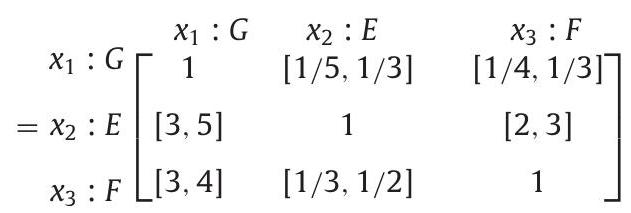
\includegraphics[max width=\textwidth]{2024_01_11_2cd5b15325412bfb985dg-03(1)}
\end{center}

As per (3.1), the constructed multiplicative comparison matrices $A_{1}^{\prime L}=\left(a_{i j}^{\prime L}\right)_{3 \times 3}$ and $A_{1}^{\prime U}=\left(a_{i j}^{\prime U}\right)_{3 \times 3}$ are determined as:

\begin{center}
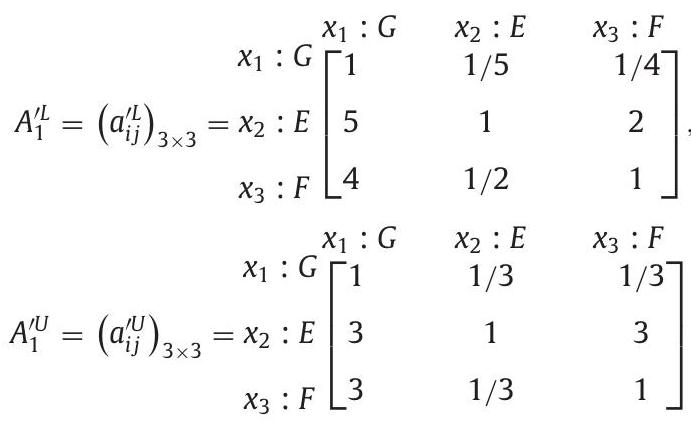
\includegraphics[max width=\textwidth]{2024_01_11_2cd5b15325412bfb985dg-03}
\end{center}

By (2.5), it is confirmed that $\operatorname{CR}\left(A_{1}^{\prime L}\right)=0.0236$ and $\operatorname{CR}\left(A_{1}^{\prime U}\right)=$ 0.1279 . Since $\mathrm{CR}\left(A_{1}^{\prime U}\right)>0.1, A_{1}^{\prime U}$ 's consistency is unacceptable. As per Liu (2009), $\bar{A}_{1}^{\prime}$ is an unacceptable IMCM. This is apparently selfcontradictory and unreasonable as both IMCMs $\bar{A}_{1}$ and $\bar{A}_{1}^{\prime}$ represent the same pair-wise comparison results with the only difference in relabeling the three alternatives.

Let $\sigma$ be a permutation of $\{1,2,3\}$ with $\sigma(1)=3, \sigma(2)=1$ and $\sigma(3)=2$, then we have $\bar{A}_{1}^{\prime}=\left(\left[a_{\sigma(i) \sigma(j)}^{-}, a_{\sigma(i) \sigma(j)}^{+}\right]\right)_{3 \times 3}$, i.e., the IMCM $\bar{A}_{1}^{\prime}$ is a permutation of $\bar{A}_{1}$. The aforesaid example clearly demonstrates the technical deficiency of the acceptable consistency proposed by Liu (2009): the judgment of an IMCM's acceptable consistency depends on how the alternatives are labeled and a new permutation with the same IMCM may lead to a contradictory result.

This analysis indicates that the existing acceptable consistency and acceptability definitions are problematic in modeling transitivity and indeterminacy in a DM's pair-wise comparison. Next, we shall introduce new acceptable consistency and acceptability definitions for IMCMs.

\section*{4. New acceptable consistency and acceptability of IMCMs}
This section first introduces an interval-arithmetic-based transitivity equation to define consistency of IMCMs. We then put forward acceptable consistency of IMCMs and a definition of indeterminacy ratio of an IMCM, thereby introducing the notion of acceptable IMCMs and defining a geometric-mean-based indeterminacy index for an IMCM. Useful properties are subsequently derived for consistent IMCMs and acceptable IMCMs.

\subsection*{4.1. Acceptable consistency of IMCMs}
Definition 4.1. Let $\bar{A}=\left(\bar{a}_{i j}\right)_{n \times n}=\left(\left[a_{i j}^{-}, a_{i j}^{+}\right]\right)_{n \times n}$ be an IMCM, if $\bar{A}$ satisfies the transitivity condition:

$\bar{a}_{i j} \otimes \bar{a}_{j k} \otimes \bar{a}_{k i}=\bar{a}_{i k} \otimes \bar{a}_{k j} \otimes \bar{a}_{j i}, \quad i, j, k=1,2, \ldots, n$

then $\bar{A}$ is called consistent.

By interval arithmetic, if all interval comparisons $\bar{a}_{i j}(i, j=$ $1,2, \ldots, n)$ in $\bar{A}$ are reduced to ratio-based crisp values, i.e., $a_{i j}^{-}=$ $a_{i j}^{+}, \forall i, j=1,2, \ldots, n$, then IMCM $\bar{A}$ is equivalent to a multiplicative comparison matrix $A=\left(a_{i j}\right)_{n \times n}$, where $a_{i j}=a_{i j}^{-}=a_{i j}^{+}$for all $i, j=$ $1,2, \ldots, n$. In this case, (4.1) is reduced to (2.3), which is equivalent to the multiplicative transitivity condition (2.2) given by Saaty (1980). Therefore, the consistency (4.1) is a natural generalization of Saaty's original multiplicative consistency.

Obviously, (4.1) is independent of the index order of $i, j, k$ and, hence, Definition 4.1 is robust when alternative labels are permutated. By Definition 4.1, $\bar{A}_{1}$ and $\bar{A}_{1}^{\prime}$ in Example 1 are two inconsistent IMCMs. Hereafter, when an IMCM is called consistent, it is always under Definition 4.1 unless otherwise stated. Similarly, whenever a multiplicative comparison matrix is referred to be consistent, it is always in terms of consistency given in Definition 2.1.

Theorem 4.1. An IMCM $\bar{A}=\left(\bar{a}_{i j}\right)_{n \times n}=\left(\left[a_{i j}^{-}, a_{i j}^{+}\right]\right)_{n \times n}$ is consistent if and only if

$a_{i k}^{-} a_{i k}^{+}=a_{i j}^{-} a_{i j}^{+} a_{j k}^{-} a_{j k}^{+}, i, j, k=1,2, \ldots, n$

Proof. Sufficiency: As per multiplicative reciprocity of IMCMs, we have $a_{i j}^{-} a_{j i}^{+}=1 \forall i, j=1,2, \ldots, n$. It follows from (4.2) that $a_{i j}^{-} a_{j k}^{-} a_{k i}^{-}=$ $a_{i k}^{-} a_{k j}^{-} a_{j i}^{-}$and $a_{i j}^{+} a_{j k}^{+} a_{k i}^{+}=a_{i k}^{+} a_{k j}^{+} a_{j i}^{+}$. By interval arithmetic described in Section 2, one can obtain

$$
\begin{aligned}
\bar{a}_{i j} \otimes \bar{a}_{j k} \otimes \bar{a}_{k i} & =\left[a_{i j}^{-} a_{j k}^{-} a_{k i}^{-}, a_{i j}^{+} a_{j k}^{+} a_{k i}^{+}\right]=\left[a_{i k}^{-} a_{k j}^{-} a_{j i}^{-}, a_{i k}^{+} a_{k j}^{+} a_{j i}^{+}\right] \\
& =\bar{a}_{i k} \otimes \bar{a}_{k j} \otimes \bar{a}_{j i} .
\end{aligned}
$$

By Definition 4.1, $\bar{A}$ is consistent.
Necessity: As $\bar{A}$ is consistent, by Definition 4.1 , we have $\bar{a}_{i j} \otimes \bar{a}_{j k} \otimes$ $\bar{a}_{k i}=\bar{a}_{i k} \otimes \bar{a}_{k j} \otimes \bar{a}_{j i}$ for all $i, j, k=1,2, \ldots, n$. By reversing the proof of sufficiency, one gets $a_{i k}^{-} a_{i k}^{+}=a_{i j}^{-} a_{i j}^{+} a_{j k}^{-} a_{j k}^{+}$for all $i, j, k=1,2, \ldots, n$. $\square$

Theorem 4.1 means that the transitivity constraint (4.1) can be equivalently formulated as a crisp arithmetic Eq. (4.2), implying Definition 4.1 is equivalent to the consistency introduced by Wang (2015a). The following theorem further indicates that (4.2) can be simplified by checking only the upper diagonal elements for consistency.

Theorem 4.2. Let $\bar{A}=\left(\bar{a}_{i j}\right)_{n \times n}=\left(\left[a_{i j}^{-}, a_{i j}^{+}\right]\right)_{n \times n}$ be any IMCM, then the following two statements are equivalent:

(i) $a_{i k}^{-} a_{i k}^{+}=a_{i j}^{-} a_{i j}^{+} a_{j k}^{-} a_{j k}^{+}, i, j, k=1,2, \ldots, n$.

(ii) $a_{i k}^{-} a_{i k}^{+}=a_{i j}^{-} a_{i j}^{+} a_{j k}^{-} a_{j k}^{+}, \quad \forall i<j<k$.

Proof. (i) $\Rightarrow$ (ii) is obvious.

(ii) $\Rightarrow$ (i). As $a_{i i}^{-}=a_{i i}^{+}=1$ and $a_{i j}^{-} a_{j i}^{+}=1$ for all $i, j=1,2, \ldots, n,(\mathrm{i})$ always holds if three or any two of indices $i, j, k$ are equal. Next, we consider the case that $i \neq j \neq k$. Six subcases may arise for distinct index orderings:

(a) $i<j<k$. In this case, (i) is identical to (ii). Thus, (i) holds.

(b) $i<k<j$. By (ii), we have $a_{i j}^{-} a_{i j}^{+}=a_{i k}^{-} a_{i k}^{+} a_{k j}^{-} a_{k j}^{+}$. Dividing $a_{k j}^{-} a_{k j}^{+}$ on both sides and applying reciprocity of $a_{k j}^{-} a_{j k}^{+}=1, \forall j, k=$ $1,2, \ldots, n$, one can obtain $a_{i k}^{-} a_{i k}^{+}=a_{i j}^{-} a_{i j}^{+} a_{j k}^{-} a_{j k}^{+}$.

(c) $j<i<k$. It follows from (ii) that $a_{j k}^{-} a_{j k}^{+}=a_{j i}^{-} a_{j i}^{+} a_{i k}^{-} a_{i k}^{+} \Rightarrow a_{j k}^{-} a_{j k}^{+}=$ $\frac{1}{a_{i j}^{+}} \frac{1}{a_{i j}^{-}} a_{i k}^{-} a_{i k}^{+} \Rightarrow a_{i k}^{-} a_{i k}^{+}=a_{i j}^{-} a_{i j}^{+} a_{j k}^{-} a_{j k}^{+}$.

Similarly, we obtain that (i) holds true for the remaining subcases: (d) $j<k<i$, (e) $k<j<i$ and (f) $k<i<j$.

Based on Theorems 4.1 and 4.2, we can directly derive the following result.

Corollary 4.1. An IMCM $\bar{A}=\left(\bar{a}_{i j}\right)_{n \times n}=\left(\left[a_{i j}^{-}, a_{i j}^{+}\right]\right)_{n \times n}$ is consistent if and only if

$a_{i k}^{-} a_{i k}^{+}=a_{i j}^{-} a_{i j}^{+} a_{j k}^{-} a_{j k}^{+}, \forall i<j<k$

Let

$p_{i j}^{L}= \begin{cases}1+\log _{a_{i j}^{+}} a_{i j}^{-} & a_{i j}^{-}>1 \\ 1+\log _{a_{i j}^{-}} a_{i j}^{+} & a_{i j}^{-}<1, a_{i j}^{+}<1, \\ 1 & \text { Otherwise }\end{cases}$

$p_{i j}^{U}= \begin{cases}1+\log _{a_{i j}^{-}} a_{i j}^{+} & a_{i j}^{-}>1 \\ 1+\log _{a_{i j}^{+}} a_{i j}^{-} & a_{i j}^{-}<1, a_{i j}^{+}<1 \\ +\infty & \text { Otherwise }\end{cases}$

$p^{L}=\max _{i, j=1,2, \ldots, n}\left\{p_{i j}^{L}\right\}, \quad p^{U}=\min _{i, j=1,2, \ldots, n}\left\{p_{i j}^{U}\right\}$

Obviously, $1 \leq p_{i j}^{L} \leq 2$ and $p_{i j}^{U} \geq 2$ for all $i, j=1,2, \ldots, n$. As per (4.5), we have $1 \leq p^{L} \leq 2$ and $p^{U} \geq 2$. Thus, $p^{L}$ and $p^{U}$ constitute a real interval $\left[p^{L}, p^{U}\right]$ containing 2 .

Let

$A(p)=\left(a_{i j}(p)\right)_{n \times n}=\left(\sqrt[p]{a_{i j}^{-} a_{i j}^{+}}\right)_{n \times n}$

where $p^{L} \leq p \leq p^{U}$. Based on Theorem 4.1, we have the following corollary.

Corollary 4.2. An IMCM $\bar{A}=\left(\bar{a}_{i j}\right)_{n \times n}=\left(\left[a_{i j}^{-}, a_{i j}^{+}\right]\right)_{n \times n}$ is consistent if and only if the multiplicative comparison matrix $A(p)$ defined by (4.6) is consistent for any $p \in\left[p^{L}, p^{U}\right]$.

Proof. As per (4.4) and (4.5), for $p \in\left[p^{L}, p^{U}\right]$, we have

$p_{i j}^{L} \leq \max _{i, j=1,2, \ldots, n}\left\{p_{i j}^{L}\right\}=p^{L} \leq p \leq p^{U}=\min _{i, j=1,2, \ldots, n}\left\{p_{i j}^{U}\right\} \leq p_{i j}^{U}, \forall i$,

$$
\begin{aligned}
& j=1,2, \ldots, n \\
\Rightarrow & p_{i j}^{L}-1 \leq p-1 \leq p_{i j}^{U}-1, \forall i, j=1,2, \ldots, n \\
\Rightarrow & (p-1) \ln a_{i j}^{-} \leq \ln a_{i j}^{+}, \ln a_{i j}^{-} \leq(p-1) \ln a_{i j}^{+}, \forall i, j=1,2, \ldots, n \\
\Rightarrow & \left(a_{i j}^{-}\right)^{p-1} \leq a_{i j}^{+}, a_{i j}^{-} \leq\left(a_{i j}^{+}\right)^{p-1}, \forall i, j=1,2, \ldots, n \\
\Rightarrow & \left(a_{i j}^{-}\right)^{p} \leq a_{i j}^{-} a_{i j}^{+} \leq\left(a_{i j}^{+}\right)^{p}, \forall i, j=1,2, \ldots, n \\
\Rightarrow & a_{i j}^{-} \leq \sqrt[p]{a_{i j}^{-} a_{i j}^{+}}=a_{i j}(p) \leq a_{i j}^{+}, \forall i, j=1,2, \ldots, n .
\end{aligned}
$$

As $1 / S \leq a_{i j}^{-} \leq a_{i j}^{+} \leq S, a_{i i}^{-}=a_{i i}^{+}=1$, it is natural that $a_{i i}(p)=1$ and $1 / S \leq a_{i j}(p) \leq S$ for all $i, j=1,2, \ldots, n$. By the reciprocity of $a_{i j}^{-} a_{j i}^{+}=$ 1 , one has $a_{i j}(p) a_{j i}(p)=\sqrt[p]{a_{i j}^{-} a_{i j}^{+}} \sqrt[p]{a_{j i}^{-} a_{j i}^{+}}=\sqrt[p]{a_{i j}^{-} a_{j i}^{+}} \sqrt[p]{a_{j i}^{-} a_{i j}^{+}}=1$. According to (2.1), $A(p)$ is a multiplicative comparison matrix for any $p \in\left[p^{L}, p^{U}\right]$.

Moreover, for each $p \in\left[p^{L}, p^{U}\right]$, we have

$$
\begin{aligned}
& a_{i k}^{-} a_{i k}^{+}=a_{i j}^{-} a_{i j}^{+} a_{j k}^{-} a_{j k}^{+} \Leftrightarrow\left(a_{i k}^{-} a_{i k}^{+}\right)^{1 / p}=\left(a_{i j}^{-} a_{i j}^{+} a_{j k}^{-} a_{j k}^{+}\right)^{1 / p} \\
& \Leftrightarrow\left(a_{i k}^{-} a_{i k}^{+}\right)^{1 / p}=\left(a_{i j}^{-} a_{i j}^{+}\right)^{1 / p}\left(a_{j k}^{-} a_{j k}^{+}\right)^{1 / p} \\
& \Leftrightarrow a_{i k}(p)=a_{i j}(p) a_{j k}(p), \quad \forall i, j, k=1,2, \ldots, n
\end{aligned}
$$

Thus, by Theorem 4.1, the proof of Corollary 4.2 is completed. $\quad \square$ Corollary 4.2 reveals that, for a consistent IMCM, there often exist numerous Saaty's consistent comparison matrices within it. Let

$A^{g m}=\left(a_{i j}^{g m}\right)_{n \times n}=\left(\sqrt{a_{i j}^{-} a_{i j}^{+}}\right)_{n \times n}$

It is obvious that $A^{g m}=A(2)$. From Corollary 4.2, the following result is directly obtained.

Corollary 4.3. An IMCM $\bar{A}=\left(\bar{a}_{i j}\right)_{n \times n}=\left(\left[a_{i j}^{-}, a_{i j}^{+}\right]\right)_{n \times n}$ is consistent if and only if the multiplicative comparison matrix $A^{g m}$ defined by (4.7) is consistent.

Corollary 4.3 specifies a particular crisp consistent comparison matrix within a consistent IMCM: each element of the crisp comparison matrix is given by the geometric mean of the upper and lower bounds of the corresponding interval judgment.

In real-world decision situations, DMs often furnish their preference over alternatives as IMCMs based on their subjective assessment and the transitivity property is not always honoured. By Corollary 4.3, the consistency of an IMCM $\bar{A}$ can be characterized by that of the associated crisp geometric mean matrix $A^{g m}$ defined by (4.7). Next, we introduce acceptable consistency of IMCMs as follows.

Definition 4.2. Let $\bar{A}=\left(\bar{a}_{i j}\right)_{n \times n}=\left(\left[a_{i j}^{-}, a_{i j}^{+}\right]\right)_{n \times n}$ be an IMCM with $1 / S \leq a_{i j}^{-}, a_{i j}^{+} \leq S, \bar{A}$ is acceptably consistent if the crisp judgment matrix $A^{g m}$ defined by (4.7) is acceptably consistent.

Definition 4.2 intentionally keeps the notion of acceptable consistency generic. Several consistency indices, such as Saaty's CI, the geometric consistency index (Crawford \& Williams, 1985), and the harmonic consistency index (Stein \& Mizzi, 2007), have been devised to measure consistency of crisp judgment matrices. Different thresholds have been proposed for checking acceptable consistency (Aguaron \& Moreno-Jimenez, 2003). Despite the fact that Saaty's CR has been criticized for yielding unreasonable consistency result with respect to the condition of order preservation (Bana e Costa \& Vansnick, 2008; Kułakowski, 2015), it remains the most widely used acceptable consistency in literature (Ishizaka \& Labib, 2011). Based on this consideration, we employ Saaty's CR to verify acceptable consistency of the multiplicative comparison matrix $A^{g m}$, i.e., $\mathrm{CR}\left(A^{g m}\right) \leq 0.1$. However, it should be stressed that our general acceptable consistency framework can be readily extended to other notions such as the aforesaid geometric and harmonic consistency indices.
Sometimes, DMs may give extremely indeterminate interval judgment such as $[1 / S, S]$ in a bipolar $[1 / S, S]$ scale with a neutral element of 1, indicating the DM's outright uncertainty about the comparison. For instance, if a DM furnishes an IMCM with all nondiagonal elements being $[1 / S, S]$, such a judgment matrix is technically consistent, but it discloses nothing about the DM's preference and does not help at all in deducing a reliable decision result (Dubois \& Prade, 2012; Durbach \& Stewart, 2012; Scholten et al., 2015; Wang \& Li, 2015). In this case, even if the IMCM is consistent or acceptably consistent, we should still treat it as unacceptable due to its high indeterminacy. Therefore, it is the authors' opinion that both the indeterminacy and consistency levels must be considered when determining acceptability of IMCMs. If an IMCM is too indeterminate or too inconsistent, it should be judged as unacceptable and returned to the DM for a revision. This holistic view differs from existing research on assessing acceptability of an IMCM: current literature tends to consider only the consistency level in line of Saaty's acceptable consistency without examining the indeterminacy level. It is inappropriate for IMCMs due to inherent indeterminacy in interval judgments.

\subsection*{4.2. Indeterminacy measurement and acceptability of IMCMS}
The interval width is often adopted to measure the indeterminacy level of an interval judgment (Entani \& Sugihara, 2012; Guo \& Tanaka 2010; Guo \& Wang 2012). However, the interval width sometimes does not properly capture the indeterminacy level of an interval judgment, especially when an element is expressed as a preference ratio. For instance, given two interval comparison ratios $\bar{a}=[2,3]$ and $\bar{b}=[1 / 6,1 / 2]$ on a $[1 / 9,9]$ scale, it is obvious that the width of $\bar{a}$ is larger than that of $\bar{b}$, but the indeterminacy level of $\bar{a}$ is smaller than that of $\bar{b}$ from a ratio perspective. To model acceptability of IMCMs, it is necessary to consider how to measure indeterminacy of a DM's interval comparison data.

Definition 4.3. Let $\bar{a}=\left[a^{-}, a^{+}\right]$be an interval comparison judgment on a bounded scale $[1 / S, S]$, then its indeterminacy ratio, denoted by $\operatorname{IR}(\bar{a})$, is defined by $a^{+} / a^{-}$, i.e.,

$\operatorname{IR}(\bar{a})=\frac{a^{+}}{a^{-}}$

Obviously, $1 \leq \operatorname{IR}(\bar{a}) \leq S^{2}$. If $a^{-}=a^{+}$, then $\operatorname{IR}(\bar{a})=1$, implying $\bar{a}$ is a crisp value without any indeterminacy. The larger the $\operatorname{IR}(\bar{a})$, the more indeterminate the judgment $\bar{a}$ is. Moreover, $\operatorname{IR}\left(\bar{a}^{c}\right)=\operatorname{IR}(\bar{a})$, where $\bar{a}^{c}$ is the reciprocal of $\bar{a}=\left[a^{-}, a^{+}\right]$, i.e., $\bar{a}^{c}=\frac{1}{\bar{a}}=\left[1 / a^{+}, 1 / a^{-}\right]$.

From (4.8), we have $\operatorname{IR}(\bar{a})=a^{+} / a^{-}=\left(a^{+}-a^{-}\right) / a^{-}+1$. It is clear that $\left(a^{+}-a^{-}\right) / a^{-}$can be regarded as a growth rate relative to the lower bound of the interval judgment. Therefore, it is relatively easy to determine an acceptable indeterminacy ratio threshold for an IMCM.

Definition 4.4. Let $\bar{A}=\left(\bar{a}_{i j}\right)_{n \times n}=\left(\left[a_{i j}^{-}, a_{i j}^{+}\right]\right)_{n \times n}$ be an IMCM and $t_{u r}\left(t_{u r} \geq 1\right)$ be an acceptable indeterminacy ratio threshold, if $\operatorname{IR}\left(\bar{a}_{i j}\right) \leq t_{u r}$ for all $i, j=1,2, \ldots, n$, and $\bar{A}$ is acceptably consistent under Definition 4.2, then $\bar{A}$ is called acceptable; otherwise, $\bar{A}$ is unacceptable.

Definition 4.4 stipulates that, for an IMCM to be acceptable, it must have both an acceptable indeterminacy level and an acceptable consistency level. An unacceptable IMCM $\bar{A}$ may contain extremely inconsistent or highly indeterminate information. In this case, the IMCM $\bar{A}$ should be returned to the DM for an update.

Based on this holistic view of acceptability for IMCMs, a consistent IMCM may be deemed unacceptable due to high indeterminacy. For instance, let $t_{u r}=5$, the IMCM with all nondiagonal elements being $[1 / 9,9]$ is consistent, but it is unacceptable due to $\operatorname{IR}\left(\bar{a}_{i j}\right)=81>$ $5=t_{u r}$ for all $i \neq j$. In essence, this acceptability notion furnishes an
important vehicle to control the quality of DMs' decision input IMCMs from two aspects: consistency and indeterminacy. It is simply not enough to be consistent; the indeterminacy has to be controlled to be within an acceptable threshold as well. This new quality control mechanism is presumably helpful for the DM to elicit more meaningful input and make better decisions.

Definition 4.5. Let $\bar{A}=\left(\bar{a}_{i j}\right)_{n \times n}$ be an IMCM with $\bar{a}_{i j}=\left[a_{i j}^{-}, a_{i j}^{+}\right]$, then a geometric-mean-based indeterminacy index of $\bar{A}$ is defined as

$\operatorname{II}(\bar{A})=\left(\prod_{i \neq j} \operatorname{IR}\left(\bar{a}_{i j}\right)\right)^{\frac{1}{n^{2}-n}}=\left(\prod_{i \neq j}\left(\frac{a_{i j}^{+}}{a_{i j}^{-}}\right)\right)^{\frac{1}{n^{2}-n}}$

It is obvious that $I I(\bar{A}) \geq 1$. If $\operatorname{II}(\bar{A})=1$, then $a_{i j}^{-}=a_{i j}^{+}$for all $i, j=1$, $2, \ldots, n$, and $\bar{a}_{i j}$ becomes a crisp value and $\bar{A}$ is thus reduced to a multiplicative comparison matrix; otherwise, $\bar{A}$ contains indeterminacy, and the greater the $I I(\bar{A})$, the more indeterminate the $\bar{A}$. Moreover, if $\bar{A}$ is an acceptable IMCM, by Definition $4.4, I I(\bar{A}) \leq t_{u r}$.

Since $a_{i j}^{-} a_{j i}^{+}=1$ and $a_{i j}^{+} a_{j i}^{-}=1$ in $\bar{A}$ for all $i,=1,2, \ldots, n$, one can get $\frac{a_{i j}^{+}}{a_{i j}^{-}}=\frac{a_{j i}^{+}}{a_{j i}^{-}}$. Thus, (4.9) can be rewritten as

$I I(\bar{A})=\left(\prod_{i<j}\left(\frac{a_{i j}^{+}}{a_{i j}^{-}}\right)\right)^{\frac{2}{n^{2}-n}}$

Eq. (4.10) allows us to use only the upper diagonal elements to determine the indeterminacy index of an IMCM.

Using the geometric mean idea, we introduce a ratio-based concept to gauge the difference between two IMCMs.

Definition 4.6. Let $\bar{A}=\left(\bar{a}_{i j}\right)_{n \times n}=\left(\left[a_{i j}^{-}, a_{i j}^{+}\right]\right)_{n \times n}$ and $\bar{B}=\left(\bar{b}_{i j}\right)_{n \times n}=$ $\left(\left[b_{i j}^{-}, b_{i j}^{+}\right]\right)_{n \times n}$ be any two IMCMs, then the difference ratio between $\bar{A}$ and $\bar{B}$ is defined as:

$\operatorname{DR}(\bar{A}, \bar{B})=\left(\prod_{i \neq j}\left(\frac{\max \left\{a_{i j}^{-}, b_{i j}^{-}\right\}}{\min \left\{a_{i j}^{-}, b_{i j}^{-}\right\}}\right)\left(\frac{\max \left\{a_{i j}^{+}, b_{i j}^{+}\right\}}{\min \left\{a_{i j}^{+}, b_{i j}^{+}\right\}}\right)\right)^{\frac{1}{2\left(n^{2}-n\right)}}$

Obviously, $\operatorname{DR}(\bar{A}, \bar{B}) \geq 1$ and $\operatorname{DR}(\bar{A}, \bar{B})=\operatorname{DR}(\bar{B}, \bar{A})$. The smaller the $\operatorname{ratioDR}(\bar{A}, \bar{B})$, the closer $\bar{A}$ is to $\bar{B}$. In particular, if $\operatorname{DR}(\bar{A}, \bar{B})=1$, $\bar{A}=\bar{B}$.

As $a_{i j}^{-} a_{j i}^{+}=1$ and $a_{i j}^{+} a_{j i}^{-}=1$ in $\bar{A}$, and $b_{i j}^{-} b_{j i}^{+}=1$ and $b_{i j}^{+} b_{j i}^{-}=1$ in $\bar{B}$ for all $i, j=1,2, \ldots, n$, another equivalent but simpler expression of $(4.11)$ is

$\operatorname{DR}(\bar{A}, \bar{B})=\left(\prod_{i<j}\left(\frac{\max \left\{a_{i j}^{-}, b_{i j}^{-}\right\}}{\min \left\{a_{i j}^{-}, b_{i j}^{-}\right\}}\right)\left(\frac{\max \left\{a_{i j}^{+}, b_{i j}^{+}\right\}}{\min \left\{a_{i j}^{+}, b_{i j}^{+}\right\}}\right)\right)^{\frac{1}{\left(n^{2}-n\right)}}$

Let $\bar{A}^{(l)}=\left(\bar{a}_{i j}^{(l)}\right)_{n \times n}=\left(\left[a_{i j}^{-(l)}, a_{i j}^{+(l)}\right]\right)_{n \times n}(l=1,2, \ldots, m)$ be $m$ IMCMs, we next introduce a geometric-mean-based formula to aggregate individual IMCMs into a group judgment.

$$
\begin{aligned}
\bar{A}^{G} & =\left(\bar{a}_{i j}^{G}\right)_{n \times n}=\left(\left[a_{i j}^{-G}, a_{i j}^{+G}\right]\right)_{n \times n} \\
& =\left(\left[\prod_{l=1}^{m}\left(a_{i j}^{-(l)}\right)^{\alpha_{l}}, \prod_{l=1}^{m}\left(a_{i j}^{+(l)}\right)^{\alpha_{l}}\right]\right)_{n \times n}
\end{aligned}
$$

where $\sum_{l=1}^{m} \alpha_{l}=1$ and $\alpha_{l} \geq 0$ for all $l=1,2, \ldots, m$.

One can easily prove that the aggregated matrix $\bar{A}^{G}$ is an IMCM. To facilitate future discussions, the following lemma is furnished.
Lemma 4.1. (Horn \& Johnson, 1985) Let $\lambda_{\max }^{T}$ be the largest eigenvalue of a positive matrix $T=\left(t_{i j}\right)_{n \times n}$, then

$\lambda_{\max }^{T}=\min _{Y \in R_{n}^{+}}\left\{\max _{1 \leq i \leq n}\left\{\sum_{j=1}^{n} t_{i j} \frac{y_{j}}{y_{i}}\right\}\right\}$

where $R_{n}^{+}=\left\{Y=\left(y_{1}, y_{2}, \ldots, y_{n}\right)^{T} \mid y_{i}>0, i=1,2, \ldots, n\right\}$.

Based on Lemma 4.1 and Definition 4.4, we have the following result.

Theorem 4.3. Let $t_{u r}\left(t_{u r} \geq 1\right)$ be an acceptable indeterminacy ratio threshold, and $\bar{A}^{(l)}=\left(\bar{a}_{i j}^{(l)}\right)_{n \times n}=\left(\left[a_{i j}^{-(l)}, a_{i j}^{+(l)}\right]\right)_{n \times n}(l=1,2, \ldots, m)$ be m IMCMs with $1 / 9 \leq a_{i j}^{-(l)} \leq a_{i j}^{+(l)} \leq 9$, then the aggregated IMCM $\bar{A}^{G}$ defined by (4.13) is acceptable if all $\bar{A}^{(l)}(l=1,2, \ldots, m)$ are acceptable.

Proof. As $\bar{A}^{(l)}$ is acceptable, we have $1 \leq \frac{a_{i j}^{+(l)}}{a_{i j}^{-(l)}} \leq t_{u r}$ for all $l=$ $1,2, \ldots, m$ and $i, j=1,2, \ldots, n$. It follows that

$$
\begin{aligned}
\left(\frac{a_{i j}^{+(l)}}{a_{i j}^{-(l)}}\right)^{\alpha_{l}} & \leq\left(t_{u r}\right)^{\alpha_{l}} \Rightarrow \prod_{l=1}^{m}\left(\frac{a_{i j}^{+(l)}}{a_{i j}^{-(l)}}\right)^{\alpha_{l}} \leq \prod_{l=1}^{m}\left(t_{u r}\right)^{\alpha_{l}} \\
& =t_{u r} \Rightarrow \frac{\prod_{l=1}^{m}\left(a_{i j}^{+(l)}\right)^{\alpha_{l}}}{\prod_{l=1}^{m}\left(a_{i j}^{-(l)}\right)^{\alpha_{l}}} \leq t_{u r} \Rightarrow \frac{a_{i j}^{+G}}{a_{i j}^{-G}} \leq t_{u r}
\end{aligned}
$$

for all $i, j=1,2, \ldots, n$.

On the other hand, as per Definition 4.4, one has $\operatorname{CR}\left(A^{(l) g m}\right) \leq$ $0.1(l=1,2, \ldots, m)$, where $A^{(l) g m}$ is defined by (4.7), i.e., $A^{(l) g m}=$ $\left(a_{i j}^{(l) g m}\right)_{n \times n}=\left(\sqrt{a_{i j}^{-(l)} a_{i j}^{+(l)}}\right)_{n \times n}$. It follows from (2.5) that $\frac{\lambda_{\max }^{(l) g m}-n}{(n-1) \operatorname{RI}(n)} \leq$ 0.1 for all $l=1,2, \ldots, m$. Since $\sum_{l=1}^{m} \alpha_{l}=1$ and $\alpha_{l} \geq 0$ for all $l=$ $1,2, \ldots, m$, one gets

$\frac{\sum_{l=1}^{m} \alpha_{l} \lambda_{\max }^{A^{(l) g m}}-n}{(n-1) \operatorname{RI}(n)} \leq 0.1$

Let $\omega^{(l)}=\left(\omega_{1}^{(l)}, \omega_{2}^{(l)}, \ldots, \omega_{n}^{(l)}\right)^{T} \quad(l=1,2, \ldots, m)$ be the normalized eigenvector corresponding to the largest eigenvalue $\lambda_{\max }^{A^{(l) g m}}$ of $A^{(l) g m} \omega=\lambda \omega$, and $d_{i j}^{(l)}=a_{i j}^{(l) g m} \frac{\omega_{j}^{(l)}}{\omega_{i}^{(l)}}$ for all $i, j=1,2, \ldots, n$, and $l=$ $1,2, \ldots, m$, then we have $\lambda_{\max }^{A^{(l) g m}}=\sum_{j=1}^{n} d_{i j}^{(l)}$ and $a_{i j}^{(l) g m}=d_{i j}^{(l)} \frac{\omega_{i}^{(l)}}{\omega_{j}^{(l)}}$.

As per (4.7) and (4.13), it is obvious that

$$
\begin{aligned}
A^{\mathrm{Ggm}} & =\left(a_{i j}^{\mathrm{Ggm}}\right)_{n \times n}=\left(\sqrt{a_{i j}^{-G} a_{i j}^{+G}}\right)_{n \times n} \\
& =\left(\prod_{l=1}^{m}\left(\sqrt{a_{i j}^{-(l)} a_{i j}^{+(l)}}\right)^{\alpha_{l}}\right)_{n \times n}=\left(\prod_{l=1}^{m}\left(a_{i j}^{(l) g m}\right)^{\alpha_{l}}\right)_{n \times n} .
\end{aligned}
$$

It follows from Lemma 4.1 that

$$
\begin{aligned}
\lambda_{\max }^{A^{\mathrm{Ggm}}} & =\min _{Y \in R_{n}^{+}}\left\{\max _{1 \leq i \leq n}\left\{\sum_{j=1}^{n} a_{i j}^{\mathrm{Ggm}} \frac{y_{j}}{y_{i}}\right\}\right\} \\
& =\min _{Y \in R_{n}^{+}}\left\{\max _{1 \leq i \leq n}\left\{\sum_{j=1}^{n}\left(\prod_{l=1}^{m}\left(a_{i j}^{(l) g m}\right)^{\alpha_{l}}\right) \frac{y_{j}}{y_{i}}\right\}\right\} \\
& =\min _{Y \in R_{n}^{+}}\left\{\max _{1 \leq i \leq n}\left\{\sum_{j=1}^{n}\left(\prod_{l=1}^{m}\left(d_{i j}^{(l)} \frac{\omega_{i}^{(l)}}{\omega_{j}^{(l)}}\right)^{\alpha_{l}}\right) \frac{y_{j}}{y_{i}}\right\}\right\}
\end{aligned}
$$

This implies that $\prod_{l=1}^{m}\left(\omega_{i}^{(l)}\right)^{\alpha_{l}}>0$ for all $i=1,2, \ldots, n$. Thus,

$$
Y^{\omega}=\left(\prod_{l=1}^{m}\left(\omega_{1}^{(l)}\right)^{\alpha_{l}}, \prod_{l=1}^{m}\left(\omega_{2}^{(l)}\right)^{\alpha_{l}}, \ldots, \prod_{l=1}^{m}\left(\omega_{n}^{(l)}\right)^{\alpha_{l}}\right)^{T} \in R_{n}^{+}
$$

Consequently,

$$
\begin{aligned}
\lambda_{\max }^{A^{\mathrm{Ggm}}} & =\min _{Y \in R_{n}^{+}}\left\{\max _{1 \leq i \leq n}\left\{\sum_{j=1}^{n}\left(\prod_{l=1}^{m}\left(d_{i j}^{(l)} \frac{\omega_{i}^{(l)}}{\omega_{j}^{(l)}}\right)^{\alpha_{l}}\right) \frac{y_{j}}{y_{i}}\right\}\right\} \\
& \leq \max _{1 \leq i \leq n}\left\{\sum_{j=1}^{n}\left\{\left(\prod_{l=1}^{m}\left(d_{i j}^{(l)} \frac{\omega_{i}^{(l)}}{\omega_{j}^{(l)}}\right)^{\alpha_{l}}\right) \frac{\prod_{l=1}^{m}\left(\omega_{j}^{(l)}\right)^{\alpha_{l}}}{\prod_{l=1}^{m}\left(\omega_{i}^{(l)}\right)^{\alpha_{l}}}\right)\right\} \\
& =\max _{1 \leq i \leq n}\left\{\sum_{j=1}^{n}\left(\prod_{l=1}^{m}\left(d_{i j}^{(l)}\right)^{\alpha_{l}}\right)\right\} \leq \max _{1 \leq i \leq n}\left\{\sum_{j=1}^{n}\left(\sum_{l=1}^{m} \alpha_{l} d_{i j}^{(l)}\right)\right\} \\
& =\max _{1 \leq i \leq n}\left\{\sum_{l=1}^{m} \alpha_{l}\left(\sum_{j=1}^{n} d_{i j}^{(l)}\right)\right\}=\sum_{l=1}^{m} \alpha_{l} \lambda_{\max }^{A^{(l) g m}}
\end{aligned}
$$

where the last inequality is confirmed because a weighted geometric mean is always no more than the corresponding weighted arithmetic mean.

As per (4.15) and (4.16), one has

$\mathrm{CR}\left(A^{\mathrm{Ggm}}\right)=\frac{\lambda_{\max }^{\mathrm{Ggm}^{\mathrm{Gg}}}-n}{(n-1) \operatorname{RI}(n)} \leq \frac{\sum_{l=1}^{m} \alpha_{l} \lambda_{\max }^{A^{(l) g m}}-n}{(n-1) \operatorname{RI}(n)} \leq 0.1$.

Therefore, $A^{G g m}$ is acceptably consistent. By Definition 4.4, the IMCM $\bar{A}^{G}$ is acceptable.

Theorem 4.3 demonstrates that the aggregation method (4.13) for $m$ acceptable IMCMs always results in an acceptable group IMCM. This implies that it is reasonable to employ (4.13) to aggregate individual IMCMs with acceptability into a collective IMCM in group decisions.

\section*{5. Elicitation and ranking of interval multiplicative weights}
This section first defines a notion of normalized acceptable interval multiplicative weights, then establishes an LLS model to elicit a normalized interval multiplicative weight vector from an acceptable IMCM. Subsequently, a geometric-mean-based method is developed for ranking interval multiplicative weights.

In a similar way to normalizing an interval additive weight vector (Wang \& Elhag, 2006), we introduce a notion of normalized interval multiplicative weights.

Definition 5.1. Let $\bar{w}=\left(\bar{w}_{1}, \ldots, \bar{w}_{n}\right)^{T}$ be an interval multiplicative weight vector satisfying $\bar{w}_{i}=\left[w_{i}^{-}, w_{i}^{+}\right]$and $0<w_{i}^{-} \leq w_{i}^{+}(i=$ $1, \ldots, n$ ), then $\bar{w}$ is called a normalized interval multiplicative weight vector if

$w_{i}^{+} \cdot \prod_{j \neq i} w_{j}^{-} \leq 1, w_{i}^{-} \cdot \prod_{j \neq i} w_{j}^{+} \geq 1, \quad i=1,2, \ldots, n$

Definition 5.2. Let $t_{u r}\left(t_{u r} \geq 1\right)$ be an acceptable indeterminacy ratio threshold, then a normalized interval multiplicative weight vector $\bar{w}$ is acceptable if it satisfies:

$\frac{w_{i}^{+} w_{j}^{+}}{w_{i}^{-} w_{j}^{-}} \leq t_{u r}, \quad i \neq j=1,2, \ldots, n$
Inequalities in (5.1) and (5.2) can be equivalently reformulated as

$\ln w_{i}^{+}+\sum_{\substack{j=1 \\ j \neq i}}^{n} \ln w_{j}^{-} \leq 0, \ln w_{i}^{-}+\sum_{\substack{j=1 \\ j \neq i}}^{n} \ln w_{j}^{+} \geq 0, \quad i=1,2, \ldots, n$

$\ln w_{i}^{+}+\ln w_{j}^{+}-\ln w_{i}^{-}-\ln w_{j}^{-} \leq \ln t_{u r}, \quad i \neq j=1,2, \ldots, n$

For an IMCM $\bar{A}=\left(\bar{a}_{i j}\right)_{n \times n}=\left(\left[a_{i j}^{-}, a_{i j}^{+}\right]\right)_{n \times n}$, if there exists an acceptable normalized interval multiplicative weight vector $\bar{w}$ such that

$a_{i j}^{-}=\frac{w_{i}^{-}}{w_{j}^{+}}, \quad a_{i j}^{+}=\frac{w_{i}^{+}}{w_{j}^{-}}, \quad i \neq j$

then it is easy to prove that $A^{g m}$ defined by (4.7) is a crisp judgment matrix with consistency. As per Corollary 4.3, the IMCM $\bar{A}$ is consistent. By (4.8), we have $\operatorname{IR}\left(\bar{a}_{i i}\right)=\frac{a_{i i}^{+}}{a_{i i}^{-}}=1, i=1,2, \ldots, n$ and $\operatorname{IR}\left(\bar{a}_{i j}\right)=$ $\frac{a_{i j}^{+}}{a_{i j}^{-}}=\frac{w_{i}^{+} w_{j}^{+}}{w_{i}^{-} w_{j}^{-}}, i \neq j$. It follows from (5.2) and $t_{u r} \geq 1$ that $\operatorname{IR}\left(\bar{a}_{i j}\right) \leq t_{u r}$ for all $i, j=1,2, \ldots, n$. According to Definition $4.4, \bar{A}$ is an acceptable IMCM with consistency.

Eq. (5.5) is equivalent to the following indeterminacy ratio and geometric-mean-based formulae.

$\sqrt{a_{i j}^{-} a_{i j}^{+}}=\sqrt{\frac{w_{i}^{-} w_{i}^{+}}{w_{j}^{-} w_{j}^{+}}}, \quad \frac{a_{i j}^{+}}{a_{i j}^{-}}=\frac{w_{i}^{+} w_{j}^{+}}{w_{i}^{-} w_{j}^{-}}, \quad i \neq j$

Eq. (5.6) can be equivalently rewritten as

$\ln a_{i j}^{-}+\ln a_{i j}^{+}=\ln w_{i}^{-}+\ln w_{i}^{+}-\ln w_{j}^{-}-\ln w_{j}^{+}, \quad i \neq j$

$\ln a_{i j}^{+}-\ln a_{i j}^{-}=\ln w_{i}^{+}+\ln w_{j}^{+}-\ln w_{i}^{-}-\ln w_{j}^{-}, \quad i \neq j$

Eqs. (5.7) and (5.8) hold only for consistent IMCMs. For an inconsistent IMCM with acceptable consistency, the equations in (5.7) and (5.8) will be relaxed by allowing deviations. The smaller the squared deviation, the closer the IMCM $\bar{A}$ is to have consistency. According to this modeling notion, the following multi-objective LLS models are developed to generate interval multiplicative weights from an acceptable IMCM $\bar{A}=\left(\bar{a}_{i j}\right)_{n \times n}=\left(\left[a_{i j}^{-}, a_{i j}^{+}\right]\right)_{n \times n}$.

$$
\begin{aligned}
\min J_{1}= & \sum_{i=1}^{n} \sum_{j \neq i, j=1}^{n}\left(\ln a_{i j}^{-}+\ln a_{i j}^{+}-\ln w_{i}^{-}\right. \\
& \left.-\ln w_{i}^{+}+\ln w_{j}^{-}+\ln w_{j}^{+}\right)^{2}
\end{aligned}
$$

$\min J_{2}=\sum_{i=1}^{n} \sum_{j \neq i, j=1}^{n}\left(\ln a_{i j}^{+}-\ln a_{i j}^{-}-\ln w_{i}^{+}\right.$

$$
\left.-\ln w_{j}^{+}+\ln w_{i}^{-}+\ln w_{j}^{-}\right)^{2}
$$

$$
\text { s.t. } \begin{cases}\ln w_{i}^{+}+\sum_{\substack{j=1 \\ j \neq i}}^{n} \ln w_{j}^{-} \leq 0, & i=1,2, \ldots, n \\ \ln w_{i}^{-}+\sum_{\substack{j=1 \\ j \neq i}}^{n} \ln w_{j}^{+} \geq 0, & i=1,2, \ldots, n \\ 0<w_{i}^{-}, \quad \ln w_{i}^{-} \leq \ln w_{i}^{+}, & i=1,2, \ldots, n \\ \ln w_{i}^{+}+\ln w_{j}^{+}-\ln w_{i}^{-}-\ln w_{j}^{-} \leq \ln t_{u r} . & i, j=1,2, \ldots, n, i \neq j\end{cases}
$$

where $t_{u r}$ is an acceptable indeterminacy ratio threshold and the first three lines of inequalities are the logarithms of the normalization
constraints for interval multiplicative weights, and the last line of the constraints is due to (5.4) and ensures the derived interval multiplicative weights to be acceptable.

Obviously, $\quad \hat{\bar{w}}=\left(\left[\hat{w}_{1}^{-}, \hat{w}_{1}^{+}\right],\left[\hat{w}_{2}^{-}, \hat{w}_{2}^{+}\right], \ldots,\left[\hat{w}_{n}^{-}, \hat{w}_{n}^{+}\right]\right)^{T}$ with $0<$ $\hat{w}_{i}^{-}=\hat{w}_{i}^{+}, i=1,2, \ldots, n$ and $\prod_{i=1}^{n} \hat{w}_{i}^{-}=1$ satisfies (5.11) for any $t_{u r} \geq$ 1 , thus it is a feasible solution to (5.9) and (5.10). Moreover, the following result can be easily proved.

Theorem 5.1. Let $\tilde{\bar{w}}=\left(\left[\tilde{w}_{1}^{-}, \tilde{w}_{1}^{+}\right],\left[\tilde{w}_{2}^{-}, \tilde{w}_{2}^{+}\right], \ldots,\left[\tilde{w}_{n}^{-}, \tilde{w}_{n}^{+}\right]\right)^{T}$ be an optimal solution of (5.9) and (5.10), then $\tilde{\bar{w}}^{\prime}=\left(\gamma\left[\tilde{w}_{1}^{-}, \tilde{w}_{1}^{+}\right]\right.$, $\left.\gamma\left[\tilde{w}_{2}^{-}, \tilde{w}_{2}^{+}\right], \ldots, \gamma\left[\tilde{w}_{n}^{-}, \tilde{w}_{n}^{+}\right]\right)^{T}$ is also an optimal solution, where the parameter $\gamma$ satisfies

$\gamma>0, \quad \gamma^{n} w_{i}^{+} \prod_{j=1, j \neq i}^{n} w_{j}^{-} \leq 1, \quad \gamma^{n} w_{i}^{-} \prod_{j=1, j \neq i}^{n} w_{j}^{+} \geq 1, \quad i=1,2, \ldots, n$

Theorem 5.1 shows that multiple solutions may exist for the multi-objective optimization models (5.9) and (5.10). To narrow down the optimal solutions and provide a benchmark, we add the following constraint into (5.11).

$\prod_{i=1}^{n} \sqrt{w_{i}^{-} w_{i}^{+}}=1$

Let

$w_{i}^{g m}=\sqrt{w_{i}^{-} w_{i}^{+}}$

we have $\ln w_{i}^{g m}=\frac{1}{2}\left(\ln w_{i}^{-}+\ln w_{i}^{+}\right)$and $\prod_{i=1}^{n} w_{i}^{g m}=1$. Therefore, a normalized geometric-mean-based benchmark is found by solving the following two LLS models:

$\min J_{1}=4 \sum_{i=1}^{n} \sum_{j \neq i, j=1}^{n}\left(\ln \left(\sqrt{a_{i j}^{-} a_{i j}^{+}}\right)-\ln w_{i}^{g m}+\ln w_{j}^{g m}\right)^{2}$

s.t. $\left\{\begin{array}{l}\prod_{i=1}^{n} w_{i}^{g m}=1, \\ w_{i}^{g m}>0 . \quad i=1,2, \ldots, n\end{array}\right.$

where $w_{i}^{g m}(i=1,2, \ldots, n)$ are decision variables.

$\min J_{2}=\sum_{i=1}^{n} \sum_{j \neq i, j=1}^{n}\left(\ln a_{i j}^{+}-\ln a_{i j}^{-}-\ln w_{i}^{+}-\ln w_{j}^{+}+\ln w_{i}^{-}+\ln w_{j}^{-}\right)^{2}$

s.t. $\begin{cases}\ln w_{i}^{+}+\sum_{\substack{j=1 \\ j \neq i}}^{n} \ln w_{j}^{-} \leq 0, & \\ \ln w_{i}^{-}+\sum_{\substack{j=1 \\ j \neq i}}^{n} \ln w_{j}^{+} \geq 0, & i=1,2, \ldots, n \\ 0<w_{i}^{-}, \quad \ln w_{i}^{-} \leq \ln w_{i}^{+}, & i=1,2, \ldots, n \\ \ln w_{i}^{-}+\ln w_{i}^{+}=2 \ln w_{i}^{g m *}, & i=1,2, \ldots, n \\ \ln w_{i}^{+}+\ln w_{j}^{+}-\ln w_{i}^{-}-\ln w_{j}^{-} \leq \ln t_{u r .} & i \neq j=1,2, \ldots, n\end{cases}$

where $\left(w_{1}^{g m *}, w_{2}^{g m *}, \ldots, w_{n}^{g m *}\right)^{T}$ is the optimal solution to (5.15), $w_{i}^{-}$ and $w_{i}^{+}(i=1,2, \ldots, n)$ are decision variables.

One can see that the LLS model (5.15) is equivalent to generating crisp multiplicative weights from the comparison matrix $A^{g m}$ defined by (4.7). According to the well known geometric mean procedure proposed by Crawford and Williams (1985), one can obtain

$w_{i}^{g m *}=\left(\prod_{k=1}^{n} \sqrt{a_{i k}^{-} a_{i k}^{+}}\right)^{1 / n}, \quad i=1,2, \ldots, n$.
On the other hand, as per the reciprocity of $a_{i j}^{-} a_{j i}^{+}=1, \forall i, j=$ $1,2, \ldots, n$, we have

$$
\begin{aligned}
& \left(\ln a_{j i}^{+}-\ln a_{j i}^{-}-\ln w_{j}^{+}-\ln w_{i}^{+}+\ln w_{j}^{-}+\ln w_{i}^{-}\right)^{2} \\
& \quad=\left(\ln a_{i j}^{+}-\ln a_{i j}^{-}-\ln w_{i}^{+}-\ln w_{j}^{+}+\ln w_{i}^{-}+\ln w_{j}^{-}\right)^{2} .
\end{aligned}
$$

Therefore, an optimal solution to (5.16) is found by solving the following optimization model:

$\min J=\sum_{i=1}^{n-1} \sum_{j=i+1}^{n}\left(\ln a_{i j}^{+}-\ln a_{i j}^{-}-\ln w_{i}^{+}-\ln w_{j}^{+}+\ln w_{i}^{-}+\ln w_{j}^{-}\right)^{2}$

$$
\text { s.t. } \begin{cases}\ln w_{i}^{+}+\sum_{\substack{j=1 \\ j \neq i}}^{n} \ln w_{j}^{-} \leq 0, & \\ \ln w_{i}^{-}+\sum_{\substack{j=1 \\ j \neq i}}^{n} \ln w_{j}^{+} \geq 0, & i=1,2, \ldots, n \\ 0<w_{i}^{-}, \quad \ln w_{i}^{-} \leq \ln w_{i}^{+}, & i=1,2, \ldots, n \\ \ln w_{i}^{-}+\ln w_{i}^{+}=\frac{1}{n} \sum_{k=1}^{n}\left(\ln a_{i k}^{-}+\ln a_{i k}^{+}\right), & i=1,2, \ldots, n \\ \ln w_{i}^{+}+\ln w_{j}^{+}-\ln w_{i}^{-}-\ln w_{j}^{-} \leq \ln t_{u r} . & i<j\end{cases}
$$

Solving (5.18) yields an optimal interval multiplicative weight vector denoted by $\bar{w}^{*}=\left(\bar{w}_{1}^{*}, \bar{w}_{2}^{*}, \ldots, \bar{w}_{n}^{*}\right)^{T}=$ $\left(\left[w_{1}^{-*}, w_{1}^{+*}\right],\left[w_{2}^{-*}, w_{2}^{+*}\right], \ldots,\left[w_{n}^{-*}, w_{n}^{+*}\right]\right)^{T}$.

If all interval comparisons of $\bar{A}=\left(\bar{a}_{i j}\right)_{n \times n}=\left(\left[a_{i j}^{-}, a_{i j}^{+}\right]\right)_{n \times n}$ are reduced to crisp ratio values, i.e., $a_{i j}^{-}=a_{i j}^{+}, \forall i, j=1,2, \ldots, n, \bar{A}$ is reduced to a crisp comparison matrix $A=\left(a_{i j}^{-}\right)_{n \times n}$. In this case, for any $t_{u r} \geq 1$, the optimal value of the objective function (5.18) is equal to zero, and we have the optimal solution $w_{i}^{-*}=w_{i}^{+*}=\left(\prod_{k=1}^{n} a_{i k}^{-}\right)^{1 / n}(i=$ $1,2, \ldots, n)$, leading to the same result derived by the geometric mean procedure by Crawford and Williams (1985).

Let

$\bar{a}_{i j}^{*}=\left[a_{i j}^{-*}, a_{i j}^{+*}\right]= \begin{cases}{[1,1]} & i=j \\ {\left[\frac{w_{i}^{-*}}{w_{j}^{+*}}, \frac{w_{i}^{*+}}{w_{j}^{-*}}\right]} & i \neq j\end{cases}$

we obtain a consistent and acceptable IMCM $\bar{A}^{*}=\left(\left[a_{i j}^{-*}, a_{i j}^{+*}\right]\right)_{n \times n}$ based on $\bar{A}$.

Once multiplicative priority weights are generated from IMCMs, the next issue is to compare them and deduce a rank. Wang et al. (2005a) and Liu (2009) developed interval midpoint-based methods to compare two interval multiplicative weights, which are equivalent to an arithmetic mean approach. To be consistent with the geometricmean-based modeling idea in this article, we introduce an alternative geometric-mean-based possibility degree formula and employ it to compare and rank interval multiplicative weights $\bar{w}_{i}=\left[w_{i}^{-}, w_{i}^{+}\right](i=$ $1,2, \ldots, n)$.

$P_{M}\left(\bar{w}_{i} \geq \bar{w}_{j}\right)=\frac{\max \left\{0, \ln w_{i}^{+}-\ln w_{j}^{-}\right\}-\max \left\{0, \ln w_{i}^{-}-\ln w_{j}^{+}\right\}}{\ln w_{i}^{+}-\ln w_{i}^{-}+\ln w_{j}^{+}-\ln w_{j}^{-}}$,

$$
\bar{w}_{i}>0, \bar{w}_{j}>0
$$

It is apparent that $P_{M}\left(\bar{w}_{i} \geq \bar{w}_{j}\right)$ satisfies the following properties:

(a) $0 \leq P_{M}\left(\bar{w}_{i} \geq \bar{w}_{j}\right) \leq 1$;

(b) $P_{M}\left(\bar{w}_{i} \geq \bar{w}_{j}\right)+P_{M}\left(\bar{w}_{j} \geq \bar{w}_{i}\right)=1$. Especially, $P_{M}\left(\bar{w}_{i} \geq \bar{w}_{i}\right)=0.5$;

(c) $P_{M}\left(\bar{w}_{i} \geq \bar{w}_{j}\right)=1 \Leftrightarrow w_{i}^{-} \geq w_{j}^{+}$;

(d) $P_{M}\left(\bar{w}_{i} \geq \bar{w}_{j}\right)=0 \Leftrightarrow w_{i}^{+} \leq w_{j}^{-}$;

(e) $P_{M}\left(\bar{w}_{i} \geq \bar{w}_{j}\right) \geq 0.5 \Leftrightarrow \sqrt{w_{i}^{-} w_{i}^{+}} \geq \sqrt{w_{j}^{-} w_{j}^{+}}$. Especially, $P_{M}\left(\bar{w}_{i} \geq\right.$

$\left.\bar{w}_{j}\right)=0.5 \Leftrightarrow \sqrt{w_{i}^{-} w_{i}^{+}}=\sqrt{w_{j}^{-} w_{j}^{+}} ;$
(f) For any three interval multiplicative weights $\bar{w}_{i}, \bar{w}_{j}$ and $\bar{w}_{k}$, if $P_{M}\left(\bar{w}_{i} \geq \bar{w}_{j}\right) \geq 0.5$ and $P_{M}\left(\bar{w}_{j} \geq \bar{w}_{k}\right) \geq 0.5$, then $P_{M}\left(\bar{w}_{i} \geq \bar{w}_{k}\right) \geq$ 0.5 .

In summary, for any acceptable IMCM $\bar{A}=\left(\bar{a}_{i j}\right)_{n \times n}=$ $\left(\left[a_{i j}^{-}, a_{i j}^{+}\right]\right)_{n \times n}$, its interval multiplicative weights are generated and ranked as per the procedure below:

(i) Solving the LLS model (5.18) to generate its optimal solution $\bar{w}_{i}^{*}=\left[w_{i}^{-*}, w_{i}^{-*}\right](i=1,2, \ldots, n)$.

(ii) Construct a possibility matrix $P=\left(p_{i j}\right)_{n \times n}=$ $\left(P_{M}\left(\bar{w}_{i}^{*} \geq \bar{w}_{j}^{*}\right)\right)_{n \times n}$ as per $(5.20)$.

(iii) Calculate ranking indices of the interval multiplicative weights $\bar{w}_{i}^{*}=\left[w_{i}^{-*}, w_{i}^{-*}\right] \quad(i=1,2, \ldots, n)$ as per the formula $\xi_{i}=$ $\sum_{j=1}^{n} p_{i j}$.

(iv) A ranking order of the decision alternatives is derived by a decreasing order of the indices $\xi_{i}(i=1,2, \ldots, n)$, and " $x_{i}$ being superior to $x_{j}$ " is denoted by $x_{i} \stackrel{P_{M}\left(\bar{\omega}_{i}^{*} \geq \bar{\omega}_{j}^{*}\right)}{\succeq} x_{j}$.

\section*{6. Numerical examples}
Next, two numerical examples are provided to illustrate the validity and applicability of the proposed models.

Example 2. Consider the following IMCM $\bar{A}_{2}$, which was examined by Liu (2009) and Wang et al. (2005a).

$$
\begin{aligned}
\bar{A}_{2} & =\left(\bar{a}_{i j}\right)_{4 \times 4}=\left(\left[a_{i j}^{-}, a_{i j}^{+}\right]\right)_{4 \times 4} \\
& =\left[\begin{array}{cccc}
1 & {[2,5]} & {[2,4]} & {[1,3]} \\
{[1 / 5,1 / 2]} & 1 & {[1,3]} & {[1,2]} \\
{[1 / 4,1 / 2]} & {[1 / 3,1]} & 1 & {[1 / 2,1]} \\
{[1 / 3,1]} & {[1 / 2,1]} & {[1,2]} & 1
\end{array}\right]
\end{aligned}
$$

Assume that an acceptable indeterminacy ratio threshold is set at $t_{u r}=3$. As per (4.8), we have $\operatorname{IR}\left(\bar{a}_{i j}\right) \leq t_{u r}$ for $i, j=$ $1,2,3,4$. By (2.5), one confirms CR $\left(A_{2}^{g m}\right)=0.0981<0.1$. According to Definition 4.4, the IMCM $\bar{A}_{2}$ is acceptable.

Plugging $\bar{A}_{2}$ into (5.18), we obtain an optimal interval multiplicative weight vector as

$\bar{w}^{*}=\left(\bar{w}_{1}^{*}, \bar{w}_{2}^{*}, \bar{w}_{3}^{*}, \bar{w}_{4}^{*}\right)^{T}=([1.5540,2.5329],[0.7348,1.1977]$,

$$
[0.5105,0.7442],[0.7219,1.0525])^{T}
$$

By (5.20), the following possibility degree matrix is established.

$P=\left[\begin{array}{cccc}0.5 & 1 & 1 & 1 \\ 0 & 0.5 & 0.9853 & 0.5849 \\ 0 & 0.0147 & 0.5 & 0.0404 \\ 0 & 0.4151 & 0.9596 & 0.5\end{array}\right]$

Consequently, we have $\xi_{1}=3.5, \xi_{2}=2.0702, \xi_{3}=0.5551, \xi_{4}=$ 1.8747, and a ranking of the four interval multiplicative weights is determined as $\bar{w}_{1}^{*}{ }^{100 \%} \bar{w}_{2}^{*} \stackrel{58.49 \%}{\succ} \bar{w}_{4}^{*} \stackrel{95.96 \%}{\succ} \bar{w}_{3}^{*}$.

This ranking order is consistent with the result given by Liu (2009) and Wang et al. (2005a). However, the possibility degrees differ. This difference is ascribed to the fact that their models use different consistent properties of IMCMs and apply different possibility degree formulae, which utilize the arithmetic means of interval multiplicative weights while our approach here adopts their geometric means.

To further validate the proposed models, a comparative analysis with the results from Liu (2009) and Wang et al. (2005a) is conducted by examining the associated consistent IMCMs generated by the obtained interval multiplicative weights.

As per (5.19), the associated consistent and acceptable IMCM is determined from the interval multiplicative weight vector $\bar{w}^{*}$ as

$\bar{A}_{2}^{*}=\left[\begin{array}{c}1 \\ {[0.2901,0.7707]} \\ {[0.2015,0.4789]} \\ {[0.2850,0.6773]}\end{array}\right.$

$[1.2975,3.4471]$
1
$[0.4262,1.0128]$

$[0.4262,1.0128]$

$[2.0881,4.9616]$

$[0.9874,2.3461]$

$[0.9700,2.0619]$

\begin{center}
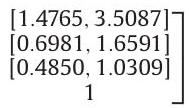
\includegraphics[max width=\textwidth]{2024_01_11_2cd5b15325412bfb985dg-09(3)}
\end{center}

By (4.9) or (4.10), the indeterminacy indices of $\bar{A}_{2}$ and $\bar{A}_{2}^{*}$ are calculated as

$I I\left(\bar{A}_{2}\right)=2.3762, \quad I I\left(\bar{A}_{2}^{*}\right)=2.3763$

As per (4.11) or (4.12), the difference ratio between $\bar{A}_{2}$ and $\bar{A}_{2}^{*}$ is determined as

$\operatorname{DR}\left(\bar{A}_{2}, \bar{A}_{2}^{*}\right)=1.2291$

From $\bar{A}_{2}$, Liu (2009) and Wang et al. (2005a) derived their interval multiplicative weight vectors $\bar{w}^{L}=\left(\bar{w}_{1}^{L}, \bar{w}_{2}^{L}, \bar{w}_{3}^{L}, \bar{w}_{4}^{L}\right)^{T}=$ ([1.4142, 2.7832], [0.8409, 1.0466], [0.5373, 0.7071], [0.6389, $1.1892])^{T}$ and $\bar{w}^{W}=\left(\bar{w}_{1}^{W}, \bar{w}_{2}^{W}, \bar{w}_{3}^{W}, \bar{w}_{4}^{W}\right)^{T}=([1.6818,2.4495]$, $[0.7598,1.1067],[0.5,0.8409],[0.6866,1])^{T}$, respectively. By applying (5.19), one can obtain their corresponding IMCMs as follows.

\begin{center}
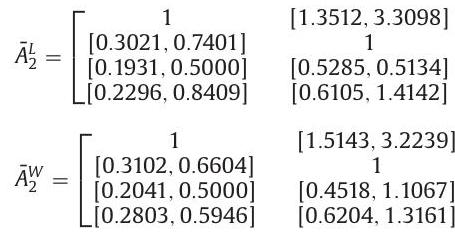
\includegraphics[max width=\textwidth]{2024_01_11_2cd5b15325412bfb985dg-09(1)}
\end{center}

\begin{center}
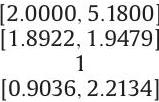
\includegraphics[max width=\textwidth]{2024_01_11_2cd5b15325412bfb985dg-09(2)}
\end{center}

$[2.0000,4.8990]$

$[0.9036,2.2134]$

[0.8165, 2.0000]

\begin{center}
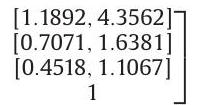
\includegraphics[max width=\textwidth]{2024_01_11_2cd5b15325412bfb985dg-09}
\end{center}

$[1.6818,3.5676]]$ $[0.7598,1.6119]$ $[0.5000,1.2247]$

As per (4.9) or (4.10), their indeterminacy indices of $\bar{A}_{2}^{L}$ and $\bar{A}_{2}^{W}$ are

$I I\left(\bar{A}_{2}^{L}\right)=2.2671, \quad I I\left(\bar{A}_{2}^{W}\right)=2.2809$

By (4.11) or (4.12), one has

$\operatorname{DR}\left(\bar{A}_{2}, \bar{A}_{2}^{L}\right)=1.3307, \quad \operatorname{DR}\left(\bar{A}_{2}, \bar{A}_{2}^{W}\right)=1.2535$

Obviously, in terms of the indeterminacy level, $\bar{A}_{2}^{*}$ is virtually identical to the original IMCM $\bar{A}_{2}$ while both $\bar{A}_{2}^{L}$ and $\bar{A}_{2}^{M}$ have a larger margin of error. Compared to $\bar{A}_{2}^{L}$ and $\bar{A}_{2}^{M}, \bar{A}_{2}^{*}$ also has the smallest difference ratio with the original IMCM. These comparative results demonstrate that the interval multiplicative weight vector $\bar{w}^{*}$ and the associated $\bar{A}_{2}^{*}$ obtained by the proposed model in this article capture the DM's original indeterminate judgments the best in terms of the indeterminacy index and difference ratio. In addition, Wang et al. (2005a) did not consider acceptability of IMCMs. While the priority method in Liu (2009) entertains acceptable consistency for IMCMs, our analysis in Section 3 indicates that the acceptable consistency therein suffers from the drawback of being sensitive to alternative label reshuffling.

Example 3. Recent rapid growth of graduate education in China creates a great need for Chinese universities to establish objective and fair criterion weighting schemes for evaluating graduate applications. It is typical to evaluate applicants based on four criteria: academic records and reputation of the undergraduate institution $\left(c_{1}\right)$, research potentials $\left(c_{2}\right)$, English proficiency and communication skills $\left(c_{3}\right)$, and teamwork $\left(c_{4}\right)$. Three experts $e_{l}(l=1,2,3)$ with an importance weight vector $\alpha=\left(\alpha_{1}, \alpha_{2}, \alpha_{3}\right)^{T}=(0.25,0.35,0.40)^{T}$ are asked to generate a proper distribution of criterion weights. Each expert $e_{l}(l=1,2,3)$ carries out pair-wise comparisons and provides his/her evaluations on the four criteria as the following IMCMs $\bar{A}^{(l)}=\left(\bar{a}_{i j}^{(l)}\right)_{4 \times 4}=\left(\left[a_{i j}^{-(l)}, a_{i j}^{+(l)}\right]\right)_{4 \times 4}$.
$\bar{A}^{(1)}=\left[\begin{array}{c}1 \\ {[1 / 2,3 / 5]} \\ {[1 / 3,3 / 4]} \\ {[2 / 3,6 / 5]}\end{array}\right.$
$[5 / 3,2]$
1
$[1 / 3,4 / 7]$
$[1 / 3,1]$
$[4 / 3,3]$
$[7 / 4,3]$
$[1 / 2,2 / 3]$
$\left.\begin{array}{c}{[5 / 6,3 / 2]} \\ {[1,3]} \\ {[3 / 2,2]} \\ 1\end{array}\right]$
$\bar{A}^{(2)}=\left[\begin{array}{c}1 \\ {[5 / 4,3}\end{array}\right]$
$[1 / 3,4 / 5$
$[4 / 3,8 / 3]$
$[3 / 2,7 / 2]$
$[3 / 8,3 / 4]$
$[1 / 4,3 / 7]$
$[7 / 3,4]$
$[4,6]$
$[1,2]$
$[1 / 2,1]$
1
$\bar{A}^{(3)}=\left[\begin{array}{cccc}1 & {[2,3]} & {[3 / 2,5 / 2]} & {[3,5]} \\ {[1 / 3,1 / 2]} & 1 & {[3 / 2,7 / 2]} & {[2,3]} \\ {[2 / 5,2 / 3]} & {[2 / 7,2 / 3]} & 1 & {[3 / 2,2]} \\ {[1 / 5,1 / 3]} & {[1 / 3,1 / 2]} & {[1 / 2,2 / 3]} & 1\end{array}\right]$

To calibrate our model, assume that the three experts agree that the acceptable indeterminacy ratio is set at $t_{u r}=3$. It follows from (4.8) that $\operatorname{IR}\left(\bar{a}_{i j}^{(l)}\right) \leq t_{u r}$ for $i, j=1,2,3,4, l=1,2,3$. As per (2.5), one can obtain $\operatorname{CR}\left(A^{(1) g m}\right)=0.0858, \operatorname{CR}\left(A^{(2) g m}\right)=0.0018$ and $\operatorname{CR}\left(A^{(3) g m}\right)=0.0521$, implying that the multiplicative comparison matrix $A^{(l) g m}$ has Saaty's acceptable consistency for $l=1,2,3$. By Definition 4.4, the three IMCMs $\bar{A}^{(l)}(l=1,2,3)$ are all acceptable.

As per the aggregation method (4.13), a group acceptable IMCM is computed as

$$
\bar{A}^{G}=\left[\begin{array}{cccc}
1 & {[1.0206,1.7068]} & {[1.3976,2.6764]} & {[1.7088,4.4132]} \\
{[0.5859,0.9798]} & 1 & {[1.8196,3.5288]} & {[2.1435,3.8237]} \\
{[0.3736,0.7155]} & {[0.2834,0.6463]} & 1 & {[1.3015,2.0000]} \\
{[0.3074,0.5852]} & {[0.2615,0.4665]} & {[0.5000,0.7683]} & 1
\end{array}\right]
$$

Solving (5.18) yields the four interval multiplicative criteria weights as follows.

$\bar{w}_{1}^{*}=[1.3151,2.0132], \quad \bar{w}_{2}^{*}=[1.3532,1.7325]$,

$\bar{w}_{3}^{*}=[0.6855,0.8716], \quad \bar{w}_{4}^{*}=[0.4625,0.6551]$.

As per (5.20), the following possibility degree matrix is obtained:

$P=\left[\begin{array}{cccc}0.5 & 0.5904 & 1 & 1 \\ 0.4096 & 0.5 & 1 & 1 \\ 0 & 0 & 0.5 & 1 \\ 0 & 0 & 0 & 0.5\end{array}\right]$

As $\xi_{1}=3.0904, \xi_{2}=2.9096, \xi_{3}=1.5, \xi_{4}=0.5$, the four criteria are ranked as $c_{1} \stackrel{59.04 \%}{\succ} c_{2} \stackrel{100 \%}{\succ} c_{3} \stackrel{100 \%}{\succ} c_{4}$.

In practice, interval criteria weights offer more decision flexibility and choices for DMs. In the context of this example, interval values can be interpreted as a general guideline for different faculties on campus. For an individual faculty, distinct real-valued weights may be derived from these interval values by assessing its specific characteristics and needs in graduate admissions.

It is noted that the approach by Liu (2009) cannot be employed to solve this group decision problem: by (2.5) and (3.1), one has $\operatorname{CR}\left(A^{(1) U}\right)=0.1161>0.1$. Thus, the IMCM $\bar{A}^{(1)}$ is deemed unacceptably inconsistent and the process has to be terminated without yielding a solution.

\section*{7. Conclusions}
This paper first shows that the acceptable consistency for IMCMs in Liu (2009) is not robust with respect to permutation of alternatives. An interval-arithmetic-based transitivity equation is then introduced to define consistency of IMCMs. By incorporating both consistency and indeterminacy levels of interval judgments, we put forward a new notion of acceptable IMCMs. Subsequently, an indeterminacy ratio of an interval comparison is introduced to define an indeterminacy index for measuring overall indeterminacy of an IMCM. We propose a notion of acceptable normalized interval multiplicative weights. An indeterminacy-ratio and geometric-mean based transformation equation is devised to convert an acceptable normalized interval multiplicative weight vector into a consistent and acceptable IMCM. An LLS model is developed to derive normalized interval multiplicative weights from an acceptable IMCM. A geometric-meanbased possibility degree is furnished for comparing and ranking normalized interval multiplicative weights. Two numerical examples are offered to demonstrate the effectiveness and applications of the proposed framework.

Future endeavors are needed to extend the paradigm for decision problems with incomplete IMCMs and addressing consensus reaching processes in group decision.

\section*{Acknowledgments}
The authors would like to thank the anonymous reviewers for their constructive comments and suggestions. The research is partially supported by the National Natural Science Foundation of China under grant nos. 71572040, 71271188, and 71272129, and the Zhejiang Provincial Natural Science Foundation of China under grant LY15G010004, and the Humanities and Social Science Foundation of Ministry of Education of China under grant 14YJC880069, and a Discovery Grant by Natural Sciences and Engineering Research Council of Canada.

\section*{References}
Aguaron, J., \& Moreno-Jimenez, J. M. (2003). The geometric consistency index: Approximated thresholds. European Journal of Operational Research, 147, 137-145.

Ahn, B. S., \& Park, H. (2014). Establishing dominance between strategies with interval judgments of state probabilities. Omega, 49, 53-59.

Bana e Costa, C. A., \& Vansnick, J. C. (2008). A critical analysis of the eigenvalue method used to derive priorities in AHP. European Journal of Operational Research, 187, $1422-1428$.

Borgonovo, E., \& Marinacci, M. (2015). Decision analysis under ambiguity. European Journal of Operational Research, 244, 823-836.

Brunelli, M., Canal, L., \& Fedrizzi, M. (2013). Inconsistency indices for pairwise comparison matrices: A numerical study. Annals of Operations Research, 211, 493-509.

Brunelli, M., \& Fedrizzi, M. (2014). Axiomatic properties of inconsistency indices for pairwise comparisons. Journal of the Operational Research Society, 66, 1-15.

Brunelli, M., \& Fedrizzi, M. (2015). Boundary properties of the inconsistency of pairwise comparisons in group decisions. European Journal of Operational Research, 240, 765773.

Crawford, G., \& Williams, C. (1985). A note on the analysis of subjective judgement matrices. Journal of Mathematical Psychology, 29, 387-405.

Dede, G., Kamalakis, T., \& Sphicopoulo, T. (2015). Convergence properties and practical estimation of the probability of rank reversal in pairwise comparisons for multicriteria decision making problems. European Journal of Operational Research, 241, $458-468$.

Dong, Y., Xu, Y., Li, H., \& Dai, M. (2008). A comparative study of the numerical scales and the prioritization methods in AHP. European Journal of Operational Research, 186, 229-242.

Dong, Y., Zhang, G., Hong, W. H., \& Xu, Y. (2010). Consensus models for AHP group decision making under row geometric mean prioritization method. Decision Support Systems, 49, 281-289.

Dubois, D. (2011). The role of fuzzy sets in decision sciences: Old techniques and new directions. Fuzzy Sets and Systems, 184, 3-28.

Dubois, D., \& Prade, H. (2012). Gradualness, uncertainty and bipolarity: Making sense of fuzzy sets. Fuzzy Sets and Systems, 192, 3-24.

Durbach, I., Lahdelma, R., \& Salminen, P. (2014). The analytic hierarchy process with stochastic judgements. European Journal of Operational Research, 238, 552-559.

Durbach, I. N., \& Stewart, T. J. (2012). Modeling uncertainty in multi-criteria decision analysis. European Journal of Operational Research, 223, 1-14.

Entani, T., \& Sugihara, K. (2012). Uncertainty index based interval assignment by Interval AHP. European Journal of Operational Research, 219, 379-385.

Entani, T., \& Tanaka, H. (2007). Interval estimations of global weights in AHP by upper approximation. Fuzzy Sets and Systems, 158, 1913-1921.

Guo, P., \& Tanaka, H. (2010). Decision making with interval probabilities. European Journal of Operational Research, 203, 444-454.

Guo, P., \& Wang, Y. (2012). Eliciting dual interval probabilities from interval comparison matrices. Information Sciences, 190, 17-26.

Horn, R. A., \& Johnson, C. R. (1985). Matrix analysis. Cambridge: Cambridge University Press.

Ishizaka, A., \& Labib, A. (2011). Review of the main developments in the analytic hierarchy process. Expert Systems with Applications, 38, 14336-14345.

Kułakowski, K. (2015). Notes on order preservation and consistency in AHP. European Journal of Operational Research, 245, 333-337.

Liu, F. (2009). Acceptable consistency analysis of interval reciprocal comparison matrices. Fuzzy Sets and Systems, 160, 2686-2700.

Merigó, J. M., Casanovas, M., \& Yang, J. B. (2014). Group decision making with expertons and uncertain generalized probabilistic weighted aggregation operators. European Journal of Operational Research, 235, 215-224.

Rezaei, J., \& Ortt, R. (2013). Multi-criteria supplier segmentation using a fuzzy preference relations based AHP. European Journal of Operational Research, 225, 75-84

Saaty, T. L. (1980). The analytic hierarchy process. New York: McGraw-Hill.

Saaty, T. L., \& Vargas, L. G. (1987). Uncertainty and rank order in the analytic hierarchy process. European Journal of Operational Research, 32, 107-117.

Scholten, L., Schuwirth, N., Reichert, P., \& Lienert, J. (2015). Tackling uncertainty in multi-criteria decision analysis - An application to water supply infrastructure planning. European Journal of Operational Research, 242, 243-260.

Siraj, S., Mikhailov, L., \& Keane, J. (2012a). A heuristic method to rectify intransitive judgments in pairwise comparison matrices. European Journal of Operational Research, 216, 420-428.

Siraj, S., Mikhailov, L., \& Keane, J. A. (2012b). Preference elicitation from inconsistent judgments using multi-objective optimization. European Journal of Operational Research, 220, 461-471.

Song, W., Ming, X., \& Xu, Z. (2013). Risk evaluation of customer integration in new product development under uncertainty. Computers \& Industrial Engineering, 65, 402412

Stein, W., \& Mizzi, P. (2007). The harmonic consistency index for the analytic hierarchy process. European Journal of Operational Research, 177, 488-497.

Sugihara, K., Ishii, H., \& Tanaka, H. (2004). Interval priorities in AHP by interval regression analysis. European Journal of Operational Research, 158, 745-754.

Wang, Y. M., \& Elhagc, T. M. S. (2006). On the normalization of interval and fuzzy weights. Fuzzy Sets and Systems, 157, 2456-2471.

Wang, Y. M., \& Elhag, T. M. S. (2007). A goal programming method for obtaining interval weights from an interval comparison matrix. European Journal of Operational Research, 177, 458-471.

Wang, Y. M., Yang, J. B., \& Xu, D. L. (2005a). A two-stage logarithmic goal programming method for generating weights from interval comparison matrices. Fuzzy Sets and Systems, 152, 475-498.

Wang, Y. M., Yang, J. B., \& Xu, D. L. (2005b). Interval weight generation approaches based on consistency test and interval comparison matrices. Applied Mathematics and Computation, 167, 252-273.

Wang, Z. J. (2015a). A note on "A goal programming model for incomplete interval multiplicative preference relations and its application in group decision-making". European Journal of Operational Research, 247, 867-871.

Wang, Z. J. (2015b). Uncertainty index based consistency measurement and priority generation with interval probabilities in the analytic hierarchy process. Computers \& Industrial Engineering, 83, 252-260.
Wang, Z. J., \& Li, K. W. (2015). A multi-step goal programming approach for group decision making with incomplete interval additive reciprocal comparison matrices. European Journal of Operational Research, 242, 890-900.

Wu, J., Li, J. C., Li, H., \& Duan, W. Q. (2009). The induced continuous ordered weighted geometric operators and their application in group decision making. Computers $\mathcal{E}$ Industrial Engineering, 56, 1545-1552.

$\mathrm{Xu}, \mathrm{Y}$. J. (2010). Note on "The induced continuous ordered weighted geometric operators and their application in group decision making". Computers \& Industrial Engineering, 59, 365-366.

$\mathrm{Xu}, \mathrm{Z.}$, \& Chen, J. (2008). Some models for deriving the priority weights from interval fuzzy preference relations. European Journal of Operational Research, 184, 266-280.

Yan, H. B., \& Ma, T. (2015). A group decision-making approach to uncertain quality function deployment based on fuzzy preference relation and fuzzy majority. European Journal of Operational Research, 241, 815-829.

Zhu, B., \& Xu, Z. (2014). Analytic hierarchy process-hesitant group decision making European Journal of Operational Research, 239, 794-801.

\begin{itemize}
  \item 
\end{itemize}


\end{document}